\documentclass[acp,manuscript]{copernicus}
\usepackage{xspace}
\usepackage{bm}

\graphicspath{{figs/}}

\newcommand*{\eg}{e.g.\@\xspace}
\newcommand*{\ie}{i.e.\@\xspace}

\newcommand{\ensSize}{\ensuremath{N_E}\xspace}
\newcommand{\latentDim}{\ensuremath{K}\xspace}
\newcommand{\spaceDim}{\ensuremath{N}\xspace}
\newcommand{\obsDim}{\ensuremath{M}\xspace}

%\includeonly{sections/conclusions}

\begin{document}

\title{Integrating generative AI with physics-based simulations for probabilistic modelling of volcanic clouds}

\Author[1][lmingari@csic.es]{Leonardo}{Mingari} %% correspondence author
\Author[1]{Arnau}{Folch}
\Author[1]{Heribert}{Pascual}
\Author[2]{Manuel}{Titos}

\affil[1]{Geosciences Barcelona (GEO3BCN-CSIC), Barcelona, Spain}
\affil[2]{University of Granada, Granada, Spain}

\runningtitle{Generative AI for volcanic cloud modelling}

\runningauthor{L. Mingari}

\received{}
\pubdiscuss{} %% only important for two-stage journals
\revised{}
\accepted{}
\published{}

\firstpage{1}

\maketitle

\begin{abstract}
%
% 1. Motivation
%
Ensemble-based modelling of the atmospheric dispersal of volcanic clouds enables more realistic forecasts by explicitly accounting for uncertainties in eruption source parameters, meteorological data, and systematic errors in transport models.
%
% 2. Problem
%
Many ensemble applications, including quantification of forecast uncertainties, data assimilation, and probabilistic hazard assessments, require a large number of members to reduce sampling errors and adequately capture probability distributions. 
%
However, the simulation and processing of large ensembles with Volcanic Ash Transport and Dispersal (VATD) models can be computationally demanding, even on high-performance computing clusters. Generative AI offers a complementary approach by representing simulated fields in a lower-dimensional latent space, enabling new samples to be generated at low computational cost and facilitating the manipulation and analysis of large ensembles.
%
% 3. Method
%
In this work, a convolutional Variational AutoEncoder (VAE) is trained on ensembles of physics-based simulations and subsequently used to generate new samples, thereby expanding the original ensemble. The learned latent-space representation is then used to test two ensemble-based data assimilation methodologies: 
(i) the Ensemble transform Kalman filter and
(ii) the Regularized bootstrap particle filter,
demonstrating the advantages of performing data assimilation in a lower-dimensional space.
%
% 4. Proof-of-concept scope
%
As a first proof of concept, the VAE is trained on two-dimensional column-mass fields, and the corresponding assimilation problem is formulated in two dimensions rather than by updating the full three-dimensional concentration state.
%
% 5. Quantitative results
%
Two numerical experiments are presented. Evaluated against a larger reference ensemble, the VAE-generated ensemble in the first experiment is found to closely reproduce probability distributions and key statistics. The Jensen--Shannon divergence decreases as the generated ensemble size exceeds that of the training ensemble, while the ensemble mean achieves a MAPE of $3.4 \pm 0.6\%$ and an RMSE of $0.20 \pm 0.03$. Although these errors are higher than those of the training ensemble (MAPE $=1.78\%$), they remain relatively low in comparison with typical forecasting errors. This is corroborated by the second experiment, in which the VAE-generated ensemble shows better agreement with satellite retrievals than the training ensemble in terms of RMSE, RMSLE, and Pearson correlation coefficient, suggesting that the generation of new samples leads to a better representation of the ensemble.
%
% 6. Implications
%
These results highlight the potential of generative AI to efficiently expand physics-based ensemble forecasts and the potential to improve forecasting skill through latent-space data assimilation.
\end{abstract}

\clearpage
\tableofcontents

\introduction 
%
% General overview
%
Operational forecasts of volcanic ash and \chem{SO_2} clouds rely on physics-based numerical simulations that yield airborne concentration fields and the corresponding aviation-hazard products. In order to produce realistic forecasts, Volcanic Ash Transport and Dispersal (VATD) models must describe several complex processes, including plume micro-scale dynamics, atmospheric long-range transport, particle sedimentation and deposition or the injection of volcanic particles and aerosols into the atmosphere. However, the complexity of the underlying physical processes, the broad range of spatial and temporal scales involved, and the uncertainties in the quantification of the emissions and meteorological fields make the modelling of volcanic clouds particularly challenging and the resulting forecasts prone to errors.
%
% Model uncertainties
%
Specifically, the so-called Eruption Source Parameters (ESPs), such as those required to estimate the vertical distribution of mass along the eruptive column, mass emission rates or particle size distributions, are recognised to be first-order contributors to model errors \citep{costa2016,poulidis2021}. In fact, the determination of the ESPs is one of the major challenges in volcanic plume modelling due to limited real-time observations, complex eruptive dynamics and the rapid variability in emission patterns.
%
% Ensemble modelling
%
Ensemble modelling is a popular approach to deal with the uncertainties associated with model parameters, the spatial distribution and time dependency of emissions or the underpinning meteorological data. Over the years, the increasing availability of High-Performance Computing (HPC) resources has facilitated significantly the use of ensemble approaches across scientific and engineering domains~\citep{wu2021}, particularly in weather forecasting~\citep{toth1997,leutbecher2008,bauer2015}.
%
% Ensemble applications: error estimation, hazards studies, data assimilation
%
Volcanic cloud forecasting has also benefited from ensemble modelling approaches, especially in areas like uncertainty quantification, hazard assessment and data assimilation. With the help of ensembles, it has been possible to characterise and quantify forecast uncertainties due to poorly constrained input parameters, model errors or uncertain weather data~\citep{stefanescu2014}, expanding upon and beyond traditional forecast products based on deterministic approaches~\citep{folch2022}.
%
This is also true for volcanic hazard assessment, another aspect of paramount importance to support long-term risk-based decision-making and short-term emergency management during volcanic crises~\citep{sandri2025}. Probabilistic hazard assessments, in particular, require estimating the probabilities that a given airspace/location will be impacted by a volcanic cloud/fallout~\citep{marzocchi2006}, and a proper probabilistic hazard assessment usually require a large number of numerical simulations \citep{madankan2014,titos2022}.
%
On the other hand, forecast errors can be reduced by incorporating observations into numerical models using ensemble-based data assimilation \citep{kalnay2003}. Data Assimilation (DA) techniques have been widely used to study and forecast geophysical systems and have been applied in a variety of research and operational settings~\citep{carrasi2018}. In particular, several ensemble-based methods have been applied to volcanic plume forecasting \citep{folch2023}, including ensemble Kalman filter methods~\citep{fu2016,fu2017,osores2020,pardini2020,mingari2022} and ensemble particle filtering \citep{zidikheri2021,zidikheri2021b}.

%
% Ensembles and computational costs
%
In all these application examples, the use of large ensembles can be computationally costly, even on HPC clusters, especially in the context of real-time services.
%
Operational forecast frameworks must accommodate ensemble sizes to the available computing resources, resulting in ensembles limited to a few tens of members and the corresponding introduction of significant sampling errors \citep{weisheimer2014,berner2017,govett2024}. 
%
% Generative AI models
%
In contrast, generative AI models have the potential to generate thousands of samples almost instantaneously at very low computational cost. In particular, Machine Learning (ML) algorithms can be trained to generate results consistent with the underlying physical laws, such as those describing atmospheric dispersion and transport of volcanic plumes.
%
Some examples of physics-informed generative models preserving the underlying governing physical laws include Physics-Informed Neural Networks (PINNs) \citep{raissi2019,kashinath2021}, Diffusion Models with physical constraints \citep{gao2023,wang2025}, and Generative Adversarial Network (GANs) augmented with conservation laws or physical constraints \citep{yang2020,tretiak2022}. Similarly, the Variarional Autoencoder or VAE~\citep{kingma2013} represents one of the most prominent examples of generative models. A VAE is a type of neural network that learns a probabilistic mapping from a high-dimensional data space to a continuous latent space, which is a lower-dimensional, compressed representation of the original data that captures its most relevant underlying features. This representation enables the reconstruction and synthesis of new states by sampling from the latent space.




%
% Applications
%
%Generative AI models for volcanic clouds constitute a promising research area with broad potential applications, ranging from volcanic-cloud detection, probabilistic forecasting, development of surrogate models for physical dispersion models, sensitivity analysis, uncertainty quantification, hazard assessment and risk analysis, and data assimilation.
%
% Latent space data assimilation
%
Several recent studies have demonstrated the benefits of using a low-dimensional latent space for data assimilation purposes \citep{pasmans2025}. For example, \citet{chen2025} trained a VAE using sea ice reanalysis data and conducted assimilation experiments with a particle-filter technique, taking advantage of a VAE to extract low-dimensional representations of sea ice physical fields. In this way, the authors significantly reduced model errors by assimilating satellite observations of sea ice concentration and thickness, demonstrating that the proposed methodology is a promising solution for nonlinear data assimilation in realistic high‐dimensional geoscience applications.
%
Alternatively, \citet{pasmans2025} proposed a variant of the ensemble transform Kalman filter~\citep{bishop2001} in which the analysis update is applied in the latent space of a VAE. In addition, they also showed that by introducing a second latent space for the observational innovations, the performance can be further improved when non-Gaussian observation errors are present.

%
% Motivation
%
Previous studies employing AI-based approaches to volcanic ash dispersion have focused primarily on the detection and segmentation of volcanic clouds in satellite imagery \citep{torrisi2024,corradino2024}. However, the use of generative AI techniques for volcanic-cloud modelling and forecasting remains largely unexplored.
%
% Objectives
%
This work introduces a generative AI framework for statistically augmenting a small ensemble of physics-based numerical simulations, thereby enriching the ensemble forecast representation. A conventional VAE is employed to generate thousands of predictions (samples) of volcanic ash concentration. Specifically, an ensemble forecast of two-dimensional mass loading, \ie vertical column mass per unit area of airborne ash, served as the training data for a convolutional neural network. The training, validation and test datasets were simulated using the VATD model FALL3D~\citep{folch2020,prata2021,folch2025}. By perturbing eruption source parameters and meteorological fields, FALL3D can produce an ensemble of simulations in a very efficient way by running a parallel job with multiple GPUs~\citep{folch2022}. As a first step, this paper focuses on characterising the statistical properties of VAE-generated ensembles and evaluating the VAE performance. Importantly, although the present study is centred on volcanic ash applications, the proposed method can be readily extended to other areas of atmospheric science, with direct applications in forecasting air pollution scenarios associated with dust storms and in modelling the transport of contaminants originating from large wildfires. The study on using the latent space for satellite DA via deep learning is postponed to a following paper.
%
% Paper structure
%
The manuscript is organised as follows. Section~\ref{sec:experiments} describes the FALL3D numerical model, the model configuration and the datasets used for training and performance evaluation. The neural network architecture is described in Sect.~\ref{sec:vae} along with a brief overview of the theoretical background behind VAEs. The results are presented in Sect.~\ref{sec:results} and the performance is evaluated in terms of different metrics. Finally, conclusions are drawn in Sect.~\ref{sec:conclusions}, where some implications of this work and possible future applications are discussed.

\section{Variational Autoencoder} \label{sec:vae}
A Variational Autoencoder (VAE) is a type of generative ML model based on a neural network architecture capable of learning an efficient and probabilistic encoding of data into a latent space of low dimensionality. By sampling vectors from the learned distribution in the latent space, a decoder can afterwards generate new and realistic data samples, even when the network was trained to encode complex and high-dimensional input data ~\citep{kingma2013}. The scheme in Fig.~\ref{fig:vae} shows a typical architecture of a VAE composed of convolutional layers. First, the encoder maps input vectors $\vec{x}$ to the parameters of a multi-dimensional probability distribution over the latent space, \eg a Gaussian with parameters $\vec{\mu}$ and $\vec{\sigma}$ (note that bold symbols denote vector quantities). Second, a vector $\vec{z}$ is sampled in the latent space and passed to the decoder, which aims to reconstruct the original input $\vec{x}$. 

\begin{figure*}[htbp]
  \centering
  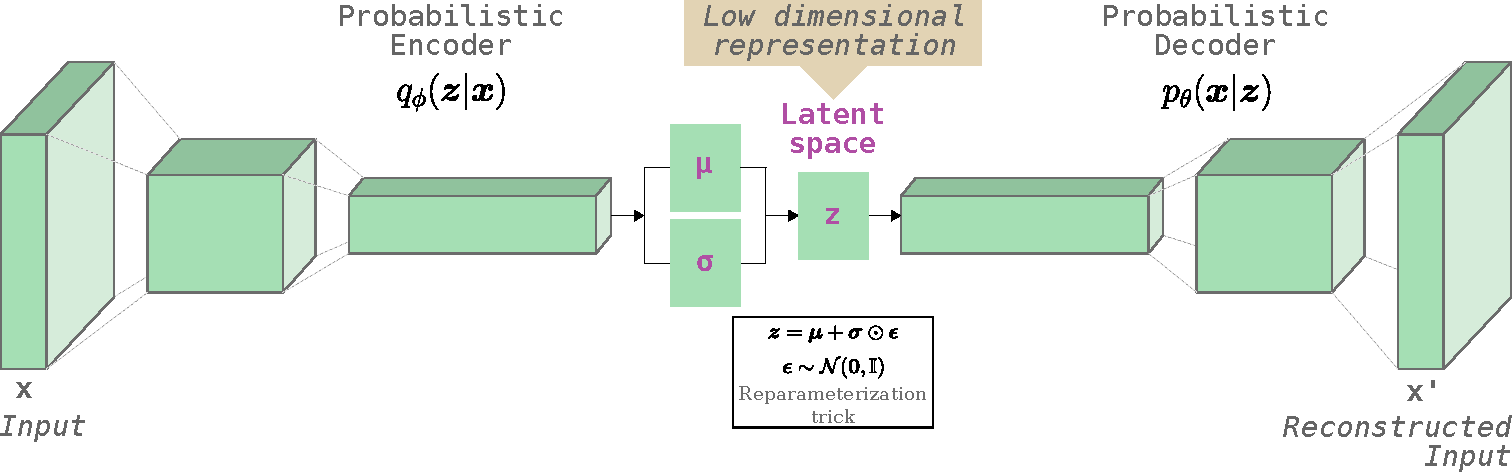
\includegraphics[width=\textwidth]{f01}
  \caption{
    The basic scheme of a VAE composed of two-dimensional convolutional layers. 
    The encoder compresses an input $\vec{x}$ into the low-dimensional latent space.
    The decoder attempts to reconstruct the original data from a vector $\vec{z}$ sampled from the latent space.
  }
  \label{fig:vae}
\end{figure*}

The training of the VAE is guided by a loss function that balances the fidelity of the data reconstruction ($\mathcal{L}_R$)  against a term that regularizes the probability distributions in the latent space towards a simple prior distribution $p(\vec{z})$ ($\mathcal{L}_{KL}$):

\begin{equation}
  \mathcal{L}_{VAE} = -\mathbb{E}_{q_{\phi}(\vec{z}\vert\vec{x})}
  \left[ \log p_{\theta}(\vec{x} \vert \vec{z}) \right] + 
  D_{KL} \left( q_{\phi}(\vec{z}\vert\vec{x}) \Vert p(\vec{z}) \right)
\label{eq:L_vae}
\end{equation}
where $q_{\phi}(\vec{z}\vert\vec{x})$ is the encoder approximate posterior and $p_{\theta}(\vec{x} \vert \vec{z})$ the decoder likelihood. Equivalently, it can be expressed as the sum of two terms:
\begin{equation*}
    \mathcal{L}_{VAE} = \mathcal{L}_R + \mathcal{L}_{KL}
\end{equation*}
The first term ($\mathcal{L}_R$, reconstruction loss) encourages reconstructions to be accurate and, in this work, it is assumed to be the Mean Squared Error (MSE) between the input ($\vec{x}$) and its reconstructed output (\vec{x}'):
\begin{equation}
  \mathcal{L}_R = \dfrac{1}{\spaceDim} \sum_{i=1}^{\spaceDim} (x_i - x'_i)^2
\end{equation}
being \spaceDim the dimension of the original space. The second term ($\mathcal{L}_{KL}$) is defined in terms of the Kullback-Leibler (KL) divergence, $D_{KL}$, and measures the distance between the approximate posterior $q_{\phi}(\vec{z} \vert \vec{x})$ and the prior distribution $p(\vec{z})$. In practice, the $D_{KL}$ term forces $q_{\phi}$ to be close to the prior distribution $p(\vec{z})$. Traditionally, the standard VAE assumes a diagonal multivariate normal distribution for the approximate posterior, $q_{\phi}(\vec{z} \vert \vec{x}) = \mathcal {N}(\vec{\mu}, \vec{\sigma^2} \mathbb{I} )$, and a standard normal distribution for the prior, $p(\vec{z}) = \mathcal {N}(\vec{0},\mathbb{I})$, leading to:
\begin{equation}
  \mathcal{L}_{KL} = -\dfrac{1}{2} \sum_{i=1}^\latentDim \left[1+\log \sigma_i^2 - \mu_i^2 - \sigma_i^2 \right]
\end{equation}
being $\vec{\mu} = (\mu_1,\dots,\mu_\latentDim)^{\intercal}$ the vector of means, $\vec{\sigma^2} = (\sigma_1^2,\dots,\sigma_\latentDim^2)$ the vector of variances and \latentDim the dimension of the latent space where vectors $\vec{z}$ live. Finally, the so-called $\beta$-VAE is a modification of the standard VAE that uses a hyperparameter $\beta$ to weight the KL divergence term in the loss function:
\begin{equation}
  \mathcal{L}_{VAE} = \mathcal{L}_R + \beta \, \mathcal{L}_{KL}
  \label{eq:vae_loss}
\end{equation}
This is the expression of the loss function used in this work. In summary, VAE training optimises the encoder and decoder by minimising the VAE loss function \eqref{eq:vae_loss} on a training set of input vectors $\left\{ \vec{x_i} \right\}$, so that inputs are accurately reconstructed from latent samples, while the latent distribution remains close to the prior.
\section{Latent-space data assimilation} 
\label{sec:da}
%
Data Assimilation (DA) techniques aim to obtain an optimal state of a dynamical system by combining model forecasts with observations, and are widely used by operational centres to forecast geophysical systems \citep{carrasi2018}. However, the application of DA to geophysical systems is challenging because their system states are typically represented by very high-dimensional vectors. As the dimensionality of a system increases, DA methods become increasingly difficult to apply due to the complexity of representing the system state and its associated uncertainties.
%
Ensemble-based DA methods partially address the issue of high-dimensionality by representing the uncertainty of the system state through a finite ensemble of model realizations. The key underpinning concept is that the ensemble can approximate the relevant error statistics, making ensemble-based methods practical for high-dimensional and non-linear geophysical systems. Still, in many geoscientific applications, the computational cost of the physical models constrains the ensemble sizes, increasing sampling errors in the estimation of ensemble statistics and potentially leading to suboptimal analyses.

These limitations are particularly relevant for atmospheric applications, where the system state may comprise millions of degrees of freedom, while non-linear dynamics and non-Gaussian error distributions can limit the applicability of traditional DA approaches. For example, many variational and Kalman filter methods rely on assumptions of approximately Gaussian error statistics, leading to inaccurate state estimates when the underlying distributions are strongly non-Gaussian.
%
Particularly challenging for DA are variables that are lower-bounded (\eg cannot take negative values) and poorly described by Gaussian distributions, such as water-vapour mixing ratios \citep{kliewer2016}, rainfall \citep{husak2007}, aerosol concentrations \citep{oneill2000}, and volcanic ash concentrations \citep{mingari2023}, often exhibiting strongly skewed and near-zero distributions.
%
Particle filters circumvent the Gaussian assumption by representing the state distribution with a set of weighted samples (particles) and updating their weights according to the observation likelihood. However, as the number of state variables grows, particle weights can collapse onto one or a few particles, leading to severe particle degeneracy.

The low-dimensional manifold learned by the VAE can be exploited to perform DA in a compressed representation of the model state, expressed in terms of a relatively small number of latent variables while retaining the main spatial structures and variability of the original fields. Thus, rather than applying DA directly to the high-dimensional ash concentration fields, the analysis is performed in the latent space, reducing the dimensionality of the problem and then using the VAE decoder to map the resulting states back to the physical space.
%
The application of ensemble-based DA methods in the VAE latent space offers several advantages. First of all, the low dimensionality of the latent representation substantially reduces the computational cost of the DA analysis, making it possible to use larger ensembles than in the original physical space. In turn, larger ensembles can potentially reduce sampling errors in the estimation of ensemble statistics. On the other hand, the compact latent representation facilitates the estimation of these statistics, while the approximately Gaussian distribution of the latent variables makes the latent space particularly suitable for ensemble-based DA methods based on Gaussian assumptions. In this work, we investigate two ensemble-based DA approaches operating in the VAE latent space: the Ensemble Transform Kalman Filter (ETKF) and the regularized bootstrap Particle Filter (PF), briefly described below.
%
% Ensemble formulation
%
\subsection{Ensemble formulation}
Let $\{ \vec{z}_i \}$ denote a prior ensemble of \ensSize latent-space vectors, with $\vec{z}_i \in \mathbb{R}^{\latentDim}$, and let $\vec{y}_{\mathrm{obs}} \in \mathbb{R}^{\obsDim}$ denote the vector of \obsDim observations. The latent-space ensemble is mapped to the physical space through the VAE decoder $D$,
%
\begin{equation}
\vec{x}_i = D(\vec{z}_i)
\end{equation}
%
with $\vec{x}_i \in \mathbb{R}^{\spaceDim}$. The corresponding observation-space ensemble is then obtained by applying the observation operator, 
%
\begin{equation}
\vec{y}_i = H(\vec{x}_i) = H(D(\vec{z}_i)),
\end{equation}
%
where $H$ is the operator mapping the physical state to the observation space. Thus, although the analysis is performed in the \latentDim-dimensional latent space, the observations are related to the latent variables through the composition of the VAE decoder and the observation operator. 

The prior ensemble mean in latent space is defined as
%
\begin{equation}
\vec{\bar{z}} = \frac{1}{\ensSize}\sum_{i=1}^{\ensSize}\vec{z}_i
\end{equation}
%
We define the background anomaly matrix $\mathbf{Z'} \in \mathbb{R}^{\latentDim \times \ensSize}$, whose $i$-th column represents the deviation of the corresponding ensemble member from the ensemble mean, $\vec{z}_i - \vec{\bar{z}}$. Similarly, we define the observation-space anomaly matrix $\mathbf{Y'} \in \mathbb{R}^{\obsDim \times \ensSize}$, whose columns represent the deviations of the observation-space ensemble members from the corresponding ensemble mean, $\vec{y}_i - \vec{\bar{y}}$.
%
% Ensemble transform Kalman filter
%
\subsection{Ensemble transform Kalman filter} \label{sec:etkf}
The Ensemble transform Kalman filter (ETKF), introduced by \cite{bishop2001}, is employed in this work following the formulation adopted by \cite{hunt2007}. The analysis ensemble is obtained by updating both the prior ensemble mean ($\vec{\bar{z}} \to \vec{\bar{z}}_a$) and the prior ensemble anomalies ($\mathbf{Z'} \to \mathbf{Z'}_a$). The analysis ensemble mean $\vec{\bar{z}}_a$ is expressed as a linear combination of the background ensemble anomalies,
%
\begin{equation}
\vec{\bar{z}}_a = \vec{\bar{z}} + \mathbf{Z'}\,\vec{w},
\label{eq:analysis_mean}
\end{equation}
%
where $\vec{w} \in \mathbb{R}^{\ensSize}$ is a vector of weights to be determined. In turn, the analysis anomalies $\mathbf{Z'}_a$ are obtained by applying a transformation matrix $\mathbf{W}$ to the background anomalies,
%
\begin{equation}
\mathbf{Z'}_a = \mathbf{Z'}\,\mathbf{W}.
\label{eq:analysis_anomalies}
\end{equation}
%
The weight vector $\vec{w}$ in \eqref{eq:analysis_mean} is obtained by
solving the linear system
\begin{equation}
\mathbf{A}\vec{w} = \mathbf{Y'}^\intercal\mathbf{R}^{-1}\vec{d},
\end{equation}
where $\mathbf{R}$ is the observation-error covariance matrix, $\vec{d} = \vec{y}_{\mathrm{obs}}-\vec{\bar{y}}$ is the innovation vector, and the matrix $\mathbf{A}$ is defined as
%
\begin{equation}
\mathbf{A} = (k-1)\mathbf{I} + \mathbf{Y'}^\intercal\mathbf{R}^{-1}\mathbf{Y'}.
\end{equation}
%
The analysis covariance in the latent space is given by
%
\begin{equation}
\mathbf{P}^a = \mathbf{Z'} \mathbf{A}^{-1} \mathbf{Z'}^\intercal
\label{eq:analysis_covariance}
\end{equation}
%
In order to obtain an ensemble with this covariance, the transformation matrix $\mathbf{W}$ in \eqref{eq:analysis_anomalies} is constructed as a symmetric square root of $(\ensSize-1)\mathbf{A}^{-1}$. Specifically, using the eigendecomposition $\mathbf{A} = \mathbf{V} \mathbf{\Lambda} \mathbf{V}^\intercal$ the transformation matrix $\mathbf{W}$ is given by
%
\begin{equation}
\mathbf{W} = \sqrt{\ensSize-1}\, \mathbf{V} \mathbf{\Lambda}^{-1/2} \mathbf{V}^\intercal
\end{equation}
%
This transformation ensures that the sample covariance of the analysis ensemble is consistent with $\mathbf{P}^a$. The posterior latent ensemble members are obtained from \eqref{eq:analysis_mean} and \eqref{eq:analysis_anomalies} by adding the transformed anomalies to the analysis mean. Finally, the resulting set of vectors $\vec{z}_a$ are then be passed through the VAE decoder to obtain the corresponding physical-space ensemble resulting from the analysis step.
%
% Regularized bootstrap particle filter
%
\subsection{Regularized bootstrap particle filter} 
\label{sec:pf}
Particle filtering \citep{doucet2001} has been successfully applied to low-dimensional models, \eg in non-linear tracking problems \citep{arulampalam2002}, but direct application of the basic PF to high-dimensional systems is prone to weight collapse, as discussed previously. As a result, several variants have been proposed to enable the application of particle filters in geophysical systems \citep{vanleeuwen2009}. Since the dimensionality of the latent space is substantially lower than that of the original physical space, we explore whether particle filtering becomes a viable option for data assimilation in this reduced representation. In this work, a basic bootstrap particle filter \citep{gordon1993} with Gaussian kernel regularization \citep{pham2001} is tested for latent-space data assimilation. The particle weights are computed from the observation likelihood,
\begin{equation}
w_i \propto p\left(\vec{y}_{\mathrm{obs}}\mid\ \vec{y}_i\right),
\end{equation}
and normalized to sum to one. The particles are then resampled according to their weights using systematic resampling \citep{kitagawa1996}, producing an equally weighted ensemble of size \ensSize. When the particle weights are highly concentrated on a small number of particles, resampling can substantially reduce the diversity of the ensemble. To restore particle diversity, the resampled particles, $\vec{z}_i^r$, are subsequently perturbed using a Gaussian kernel,
\begin{equation}
\vec{z}_i^{a}=\vec{z}_i^r+\vec{\epsilon}_i, \qquad
\vec{\epsilon}_i\sim\mathcal{N}(\vec{0},\mathbf{\Sigma}_{\mathrm{reg}}),
\end{equation}
where $\mathbf{\Sigma}_{\mathrm{reg}}=h^2\mathbf{P}$, with $\mathbf{P}$ the sample covariance of the prior latent ensemble and $h$ a prescribed regularization factor. This kernel perturbation provides a simple regularization aimed at increasing the diversity among the resampled particles.
\section{Numerical experiments and evaluation} \label{sec:experiments}
Two types of numerical experiments were performed: (i) a synthetic experiment \citep{mingari2026supplementary-synthetic} to characterize the VAE-generated ensemble and assess its ability to reproduce the statistics of a physics-based reference ensemble; and (ii) a second experiment \citep{mingari2026supplementary-etna} considering a real-case application aimed at improving the modelling of volcanic clouds through data assimilation in the latent space. The code and the material required to reproduce both experiments are available in the Supplementary Material.

\subsection{Physics-based atmospheric dispersal model}
The latest release (version 9.1) of the open-source code FALL3D \citep{folch2025} was used to produce an ensemble of numerical simulations for the two experiments. The resulting datasets were then used for VAE training, testing and evaluation. FALL3D is an Eulerian model for atmospheric passive transport and deposition of different atmospheric species (\eg, volcanic ash and gases, mineral dust and radionuclides) based on the so-called Advection-Diffusion-Sedimentation (ADS) equation \citep{folch2020,prata2021}. The numerical model is GPU-accelerated using the OpenACC parallel programming model and has been designed to support increasingly larger scientific workloads in preparation for the transition to extreme-scale computing systems \citep{folch2023b}. The FALL3D model has been deployed and optimised on several EuroHPC supercomputing systems: LUMI (Finland), Leonardo (Italy), and MareNostrum-5 (Spain), covering both NVIDIA and AMD GPU architectures.
%
FALL3D is designed to run ensemble simulations as a single, massively parallel job, allowing to maximize computational efficiency and scalability \citep{folch2022}. Broadly speaking, ensemble modelling allows to characterise and quantify model uncertainties due to poorly constrained input parameters and errors in the numerical model, physical parameterisations or underlying model-driving meteorological data. In addition, the ability to generate ensemble runs makes it possible to improve forecasts by incorporating observations using different ensemble-based data assimilation techniques. The configuration of the FALL3D model for the two experiments is summarised in Table~\ref{tab:model}. 
%
% Synthetic experiment
%
\subsection{Synthetic experiment} \label{sec:synthetic-experiment}
To define the first experiment, we used model data from the recent EU-MODEX Tenerife 2025 exercise \citep{european_commission2025}, organised under the European Civil Protection Mechanism. This exercise represented the first large-scale volcanic eruption drill in Spain to practice the response to a potential volcanic eruption from Garachico volcano (Tenerife, Canary Islands) and test the evacuation, the social assistance and communication protocols during a volcanic crisis. On 26 September 2025, we provided real-time ash-dispersion forecasts for a hypothetical eruption scenario to support emergency decision-making. Here we use the resulting simulations to characterize the statistical properties of an augmented ensemble generated by the VAE in a controlled experiment. In this context, the drill scenario refers to a fictitious eruption defined by given emission source parameters (eruption column height, mass eruption rate, and timing), rather than being constrained by real-time observations as would happen during a real event. Since our study focuses on generating ensembles from numerical simulations and approximating their statistical distribution, the distinction between real and hypothetical eruption scenarios does not affect the methodology or conclusions. This case was deliberately selected because the ensemble simulations produce qualitatively different plume transport patterns, providing a suitable test bed to inspect the ability of the VAE to reproduce the variability and statistical characteristics of the simulated ensemble.

Three ensembles were simulated with FALL3D to produce the training, validation, and test datasets. The training ensemble, consisting of 256 members, was used to train the VAE and the validation ensemble, consisting of 64 members, was used during the training step to monitor the performance and tuning of the neural network hyper-parameters. Finally, the larger test ensemble, consisting of 2048 members, was used only at the end as a purely physics-based reference to evaluate the VAE model, providing a fair (unbiased) report of model accuracy. All numerical simulations were performed on the LUMI  supercomputing system, hosted at the Finish CSC. In particular, the execution of the test ensemble required substantial HPC resources and was executed on the LUMI-G partition allocating 256 computing nodes and a total of 2048 GPUs (one per ensemble member).
%
In all cases, a 24-h time window forecast was performed assuming a continuous ash emission starting at 09:00~UTC (see Table~\ref{tab:model}), a local-scale computational domain with a horizontal resolution of $0.1\degree$ and $120 \times 100 \times 25$ grid cells, and the FALL3D dispersal model was driven by the Global Forecast System (GFS) weather forecast from the National Centers for Environmental Prediction (NCEP).
%
% Ensemble configuration
%
Each ensemble was simulated by perturbing Eruption Source Parameters (ESPs) and wind components, which are widely recognized as among the most sensitive parameters/inputs for volcanic ash transport models \citep{devenish2012,poulidis2018}. The column height was sampled around a central value of 9~\unit{km} above the vent level. Further details on the perturbed parameters and sampling ranges are provided in the Supplementary Material.

\begin{table}[htbp]
    \caption{FALL3D model configurations used in the numerical experiments.}
    \label{tab:model}
    \begin{tabular}{lcc}
    \tophline
    Parameter & Synthetic experiment & Etna experiment \\ \middlehline
    Start time & 26 September 2025 09:00~UTC & 24 December 2018 10:00~UTC \\
    Run time & 24~h & 8~h \\
    Horizontal grid resolution & 0.1\degree $\times$ 0.1\degree & 0.02\degree $\times$ 0.03\degree \\
    Grid size & 120$\times$100 & 256$\times$128 \\
    Vertical levels & 25 & 40 \\
    Grain size distribution & bi-Gaussian & bi-Gaussian \\
    Emission source & Suzuki source$^\dagger$ & Suzuki source$^\dagger$ \\
    Mass emission rate & Estimated$^\ddagger$ & Custom \\
    Ensemble size & 256 (train), 64 (validation), 2048 (test) & 128 (train), 48 (validation) \\
    \bottomhline
    \end{tabular}
    \belowtable{%
      $\dagger$ Suzuki source formulation following \citet{pfeiffer2005};
      $\ddagger$ Mass emission rate computed following
      \citet{woodhouse2016}.
      }
\end{table}

\subsection{Etna experiment} \label{sec:etna-experiment}
%
% Numerical simulations
%
The second experiment explores the feasibility of the latent-space DA using a VAE-generated prior ensemble for the 24 December 2018 Etna eruption \citep{corradini2020,pardini2020}. In this case, the FALL3D model was driven by the Copernicus regional reanalysis for Europe \citep[CERRA;][]{schimanke2021,ridal2024}, with 106 vertical model levels, and initialized at 10:00~UTC. An 8-h time window forecast was performed using a 128-member ensemble (model prior). An additional 48-member ensemble was simulated to be used as a validation dataset during the training process (see Table~\ref{tab:model}). Each ensemble was simulated by perturbing the eruptive column-top height and wind components by 20\% (see Supplementary Material for further details).

%
% VAE
%
The 128-member model prior was used to train a new VAE, which was subsequently used to sample a 4096-members ensemble (VAE prior) for the analysis step. As a proof-of-concept, we used two-dimensional ash column-mass fields rather than the full three-dimensional concentration field, both to reduce the dimensionality of the problem and to maintain a consistent neural-network architecture throughout the study. The input training data, defined on a $256 \times 128$ grid ($\spaceDim=131072$), was encoded into 32-dimensional latent space vectors. Before normalization, a $\log(1+x)$ transformation was applied to the ash column mass ($\mathbf{x}$) to reduce the strong positive skewness of its distribution, with $\mathbf{x}$ expressed in \unit{mg~m^{-2}}.

%
% Satellite
%
A single analysis step at 18:00~UTC was performed by assimilating Spinning Enhanced Visible and Infra-Red Imager (SEVIRI) volcanic ash retrievals \citep{corradini2020,corradini2021} considering two ensemble-based approaches, \ie, the ETKF (Sect.~\ref{sec:etkf}) and the PF (Sect.~\ref{sec:pf}). Only positive retrievals were considered, resulting in 2678 valid observations of ash column mass. A diagonal observation-error covariance matrix was assumed, with the observation-error standard deviation set to 50\% of the retrieved ash column mass, subject to a minimum value of 100~\unit{mg\,m^{-2}}, representative of a typical instrument detection limit.
%
% VAE configuration
%
\subsection{VAE configuration}
\label{sec:VAE_configuration}
A VAE was implemented in the PyTorch framework~\citep{paszke2019} using an architecture based on two-dimensional convolutional layers with kernel size of $3\times 3$. The VAE configuration is defined by the hyperparameters reported in Table~\ref{tab:hyperparameters}. The resulting number of trainable parameters was 698,849 and 1,783,489 for the synthetic and the Etna experiments respectively. The neural network was trained using the Adam optimizer during 400 epochs using mini-batches of 16 samples. The reconstruction loss and KL divergence (averaged over batches) were monitored at each epoch for both the training and validation datasets to prevent overfitting. Training was performed using the simulated ensembles of two-dimensional volcanic ash column-mass fields at a single forecast time. As outlined in Fig.~\ref{fig:vae}, the encoder network maps the input data $\vec{x}$ through successive convolutional layers, followed by a flattening operation to two distinct latent space parameter vectors $\vec{\mu}$ (mean) and $\log\vec{\sigma}^2$ (log-variance), with dimensions $\latentDim=16$ and $\latentDim=32$ for the synthetic and Etna experiments, respectively. The decoder then reconstructs the input from the sampled latent vector $\vec{z}$ using a fully connected layer followed by successive upsampling and convolutional operations, restoring the original spatial dimensions. For the synthetic experiment, transposed convolutional layers are used for upsampling, whereas bilinear interpolation followed by convolutional layers is used in the Etna experiment to reduce checkerboard artifacts.

\begin{table}[t]
  \caption{Hyper-parameters used for the VAE training in the synthetic and Etna experiments.}
  \label{tab:hyperparameters}
  \begin{tabular}{lcc}
    \tophline
    Hyperparameter & Synthetic & Etna \\ \middlehline
    Latent dimension \latentDim & 16 & 32 \\
    Input data size & 120$\times$100 & 256$\times$128 \\
    Number of epochs & 400 & 400 \\
    Batch size & 16 & 16 \\ 
    Convolutional layers & 6 & 8 \\
    Output channels & 16, 32, 64 & 16, 32, 64, 128 \\
    Kernel size & 3$\times$3 & 3$\times$3 \\
    Stride & 1$\times$1 & 2$\times$2 \\
    Activation function & ReLU & ReLU/Softplus \\
    Learning rate & 1E-3 & 1E-3 \\
    Optimizer & Adam & Adam \\
    Normalization & Percentile-based scaling & Logarithmic scaling \\
    \bottomhline
  \end{tabular}
\end{table}
%
% Evaluation metrics
% 
\subsection{Evaluation metrics} \label{sec:metrics}
\subsubsection{Standard performance metrics}
The performance of the generated ensembles is evaluated in terms of a set of statistical metrics. Let $\vec{x}$ and $\hat{\vec{x}}$ denote the reference and estimated quantities, respectively, with $N$ denoting the total number of values being compared. The root mean square error (RMSE) is defined as
%
\begin{equation}
  \text{RMSE} = \sqrt {\frac{1}{N}\sum^N_{j=1} (x_j-\hat{x}_j)^2}.
  \label{eq:rmse}
\end{equation}
%
The root mean square logarithmic error (RMSLE) is computed analogously after applying the logarithmic transformation $\log(1+x)$, providing a metric more sensitive to errors across multiple orders of magnitude. Similarly, the Mean Bias Error (MBE) is computed as
\begin{equation}
  \text{MBE} =\frac{1}{N}\sum^N_{j=1} x_j-\hat{x}_j
  \label{eq:mbe}
\end{equation}
The Mean Absolute Percentage Error (MAPE) provides another relative measure of accuracy:
\begin{equation}
  \text{MAPE} = 100 \times \sum^N_{j=1} \left\vert \dfrac{x_j - \hat{x}_j}{\hat{x}_j} \right\vert
  \label{eq:mape}
\end{equation}
Finally, the Pearson correlation coefficient measures the linear correlation between the estimated and reference fields.
%
% Distributional assessment
% 
\subsubsection{Distributional assessment}
In addition to the standard performance metrics introduced above, the ability of the VAE to reproduce the statistical properties of the target distribution is further assessed using distributional and spectral metrics. The Jensen-Shannon (JS) divergence is a measure of the similarity between two probability distributions. Specifically, for two distributions $P = \{p_i\}$ and $Q=\{q_i\}$, the JS divergence is a symmetrized version of the KL divergence:
\begin{equation}
  JSD(P \Vert Q) = \dfrac{1}{2} D_{KL}(P \Vert M) + \dfrac{1}{2} D_{KL}(Q \Vert M)
  \label{eq:js}
\end{equation}
where $M=\frac{1}{2}(P+Q)$ is a mixture distribution of $P$ and $Q$, while $D_{KL}$ can be interpreted as the expected logarithmic difference between the probability distributions \citep{goodfellow2016}:
\begin{equation}
  D_{KL}(P \Vert Q) = \sum p_i \log \dfrac{p_i}{q_i}
  \label{eq:kl}
\end{equation}
The discrete distributions in \eqref{eq:kl} are estimated from histograms in this work.

The two-dimensional isotropic power spectrum, $P(k)$, was also computed to assess the ability of the VAE to generate realistic samples over different spatial scales, in consistency with physically-based models. This power spectrum is defined as the radially-averaged 2D Power Spectrum Density (PSD) and is a function of the wavenumber magnitude, $k$:
\begin{equation}
  P(k) = \dfrac{1}{N_k} \sum PSD(k_x,k_y)
  \label{eq:psd}
\end{equation}
where $k=\sqrt{k_x^2 + k_y^2}$ is the magnitude of the wavevector, $PSD(k_x,k_y)$ is the two-dimensional Power Spectral Density obtained from a Fast Fourier Transform (FFT), and $N_k$ is the number of data points within an annular ring around $k$ in the Fourier space.

\subsubsection{Categorical metrics}
Categorical metrics were also used to assess binary plume detection. A positive detection is defined when the ash column mass exceeds a given threshold, set to 100~\unit{mg\,m^{-2}} in this work for demonstration purposes, which is a typical value corresponding to the satellite detection limit for ash clouds. The probability of detection (POD) measures the fraction of observed plume grid points that are correctly identified,
\begin{equation}
\mathrm{POD} = \frac{\mathrm{TP}}{\mathrm{TP}+\mathrm{FN}},
\end{equation}
where $\mathrm{TP}$ and $\mathrm{FN}$ denote true positives and false negatives, respectively. The Jaccard index measures the spatial overlap between the plume masks,
\begin{equation}
J = \frac{\mathrm{TP}}{\mathrm{TP}+\mathrm{FP}+\mathrm{FN}},
\end{equation}
where $\mathrm{FP}$ denotes false positives. In summary, the probability of detection (POD) and Jaccard index were used to quantify the detection skill and spatial overlap, respectively.

\section{Results and discussion} \label{sec:results}
The results are organized in three parts. First, the synthetic experiment is used to assess the consistency of VAE training as well as to perform a sensitivity study to select an appropriate configuration (Sect.~\ref{sec:res:training}). The selected VAE configuration is then evaluated in terms of its ability to reproduce the statistical properties of the ensemble simulated by the dispersal model (Sect.~\ref{sec:res:evaluation}). For this purpose, a large test dataset comprising 2048 simulations was generated by FALL3D in the synthetic experiment, serving as a reference for evaluating the VAE-generated ensemble.  Finally, the Etna experiment demonstrates one possible application of this methodology to a real volcanic-cloud case: the latent-space assimilation of satellite observations (Sect.~\ref{sec:res:da}). The implications of these results and the main limitations of the proposed approach are discussed in Sect.~\ref{sec:discussion}.

\subsection{Training sensitivity analysis} \label{sec:res:training}
A sensitivity analysis was conducted to evaluate the performance of different neural network configurations trained with the synthetic experiment datasets. Multiple VAE configurations were trained by exploring a range of values for two key hyperparameters: the latent space dimension \latentDim and the factor $\beta$ in \eqref{eq:vae_loss}, while fixing the remaining hyperparameters with the values specified in Table~\ref{tab:hyperparameters}.
%
% VAE generation
%
For each trained VAE, an ensemble was generated by independently sampling latent vectors from the standard normal distribution and decoding them to recover the corresponding physical-space variables. In this section, each generated ensemble consisted of 2048 members.

%
% Multi-ensemble metrics
%
The performance was evaluated in terms of the RMSE using~\eqref{eq:rmse}, computed between the ensemble mean of the test dataset (taken as the reference) and the mean of the VAE-generated ensemble. To account for the stochastic variability of the VAE generation, 20 ensembles were generated for each combination of hyperparameters tested. The resulting RMSE values are shown as boxplots in Fig.~\ref{fig:boxplot}.
%
% Optimal hyperparameters
%
In all cases, the network was trained for 400 epochs, except for configurations with latent dimensions of $\latentDim=4$ and $\latentDim=2$, where early stopping was required to avoid overfitting. According to the trend suggested by Fig.~\ref{fig:boxplot}, the best performance is achieved for latent dimensions $\latentDim \gtrsim 6$ and $\beta\gtrsim 6$. Remarkably, performance degrades slightly for large latent space dimensions (Fig.~\ref{fig:boxplot}a). There are two possible explanations for this anomaly.
%
% Latent dimension discussion
%
First, large latent spaces often produce less stable training dynamics and worse generalization: enlarging latent spaces introduces more degrees of freedom than the data can realistically support. When the dimensionality grows beyond what is needed to represent the underlying factors, the model may spread information across latent variables in an inefficient way. This leads to poor compression, weaker regularization and a latent representation that becomes harder to structure during training, limiting the extraction of compact and meaningful representations. As a result, the decoder receives a less informative latent code, reducing the reconstruction quality. On the other hand, increasing the latent dimensionality can slow convergence: since the model must explore a much larger parameter space before reaching a stable configuration, it requires more training iterations and makes optimisation more difficult.

%
% Beta discussion
%
In addition, Fig.~\ref{fig:boxplot} shows the impact of the $\beta$ parameter, which controls the strength of the KL regularization in the loss function and, therefore, the balance between reconstruction fidelity and latent-space structure. Higher values force the model to impose a tighter, more organised latent space, at the expense of losing some fine-scale details in the reconstructions. In our case, $\beta \approx 6$ suggests that a strongly regularised latent representation is more beneficial for the task than capturing every small feature in the input data. This indicates that the model gains more from enforcing a well-structured latent space than from preserving high-resolution details during reconstruction.

\begin{figure}[htbp]
  \centering
  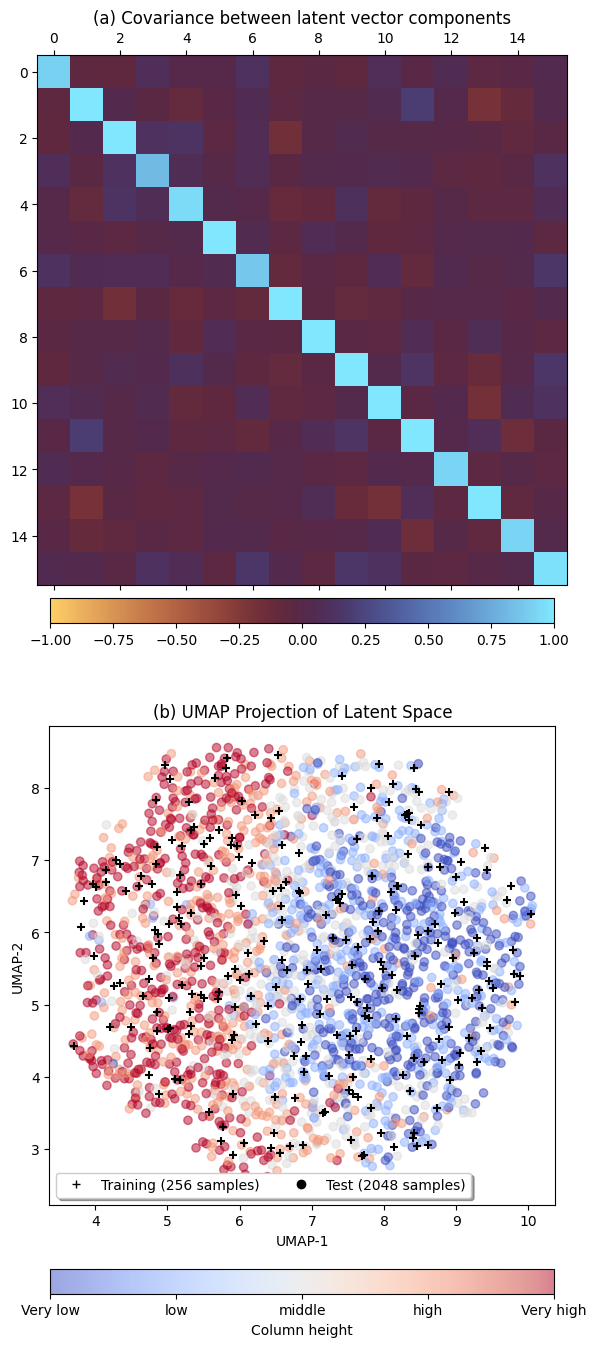
\includegraphics[width=0.4\textwidth]{f02}
  \caption{
  VAE sensitivity analysis for different combinations of two hyperparameters: the latent space dimension \latentDim (top) and the $\beta$ parameter (bottom), defined in \eqref{eq:L_vae}. 
  The performance is measured in terms of the Root-Mean-Square Error (RMSE), computed from the ensemble mean.
  }
  \label{fig:boxplot}
\end{figure}

%
% Latent space
%
This is further supported by the structure of the latent space shown in Fig.~\ref{fig:latent_space}. The nearly diagonal covariance matrix (Fig.~\ref{fig:latent_space}a) indicates weak correlation between the latent components, consistent with a well-regularized latent representation. Figure~\ref{fig:latent_space}b shows a two-dimensional visualization of the latent space based on the Uniform Manifold Approximation and Projection (UMAP) algorithm~\citep{mcinnes2020}, a technique for non-linear dimensionality reduction specifically designed to preserve the local structure of the data. The UMAP projection shows that the test dataset (circular markers) occupy the same region of latent space as the training data (plus-shaped markers), indicating that the learned representation generalizes to unseen data, rather than only organizing the training samples.
%
In addition, it is also worth showing how the encoding can discriminate between qualitatively different model solutions (ensemble members) by grouping them in different regions of the latent space. This is illustrated in Fig.~\ref{fig:latent_space}b by means of coloured-scale dots, where members with eruption column heights higher and lower than the reference (ensemble central member) are clearly concentrated in disjoint (\ie non-overlapping) regions of latent space. In other words, the VAE encoding implicitly produces a latent space with clustering-like structure.
%
% Conclusion
%
These results indicate that the network was trained correctly and behaves as expected. Based on this sensitivity analysis, a latent dimension of $\latentDim=16$ and $\beta=6$ were adopted for the VAE configuration used in the next section.

\begin{figure}[htbp]
  \centering
  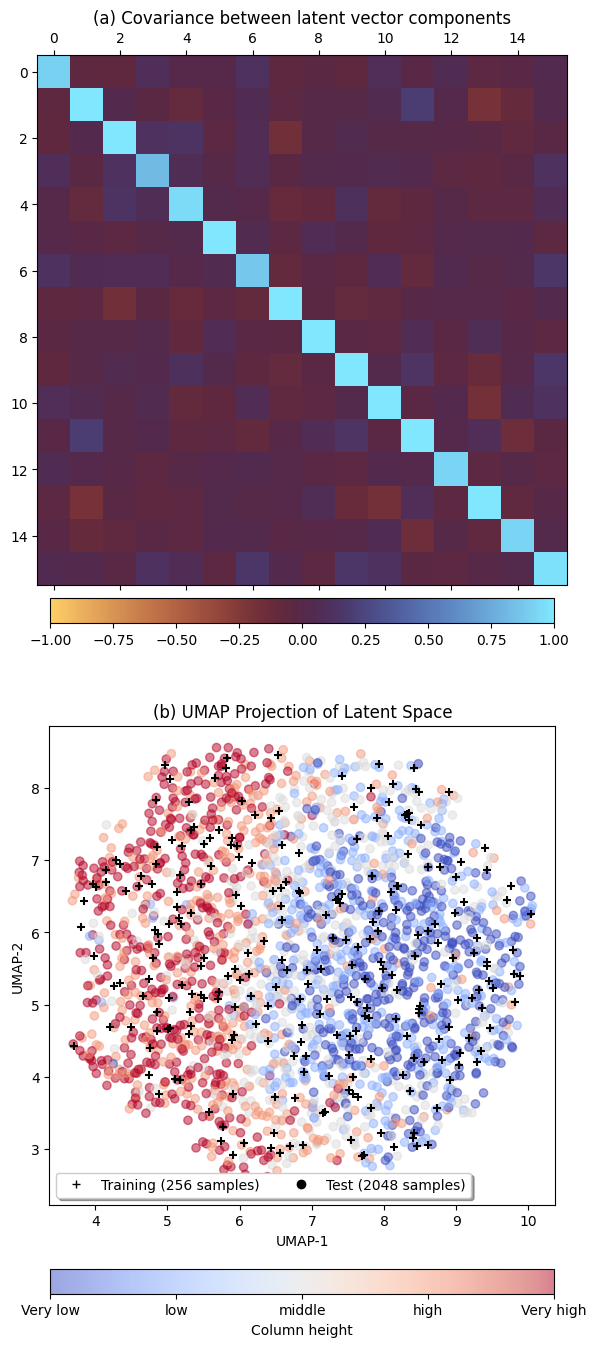
\includegraphics[width=0.4\textwidth]{f03}
  \caption{%
    Structure of the latent space. %
    The independence between the distributions of the latent vector components can be confirmed from the covariance matrix (a). 
    The test dataset is encoded in the same region of the latent space covered by the training dataset, as shown in the UMAP two-dimensional visualization of the latent space (b), confirming that the learned representation generalizes well to unseen data.
    }
  \label{fig:latent_space}
\end{figure}

\subsection{Evaluation of the VAE-generated ensemble} \label{sec:res:evaluation}
Once the VAE neural network has been trained with numerical simulations, new samples can be generated at very low computational cost. In this section, we explore whether these samples can reproduce the statistical characteristics of an independent and larger ensemble of numerical simulations (test dataset from the synthetic experiment), even when the new samples have not been obtained by explicitly solving the underlying physical equations.
%
% VAE-generated ensemble in the physical space
%
For illustrative purposes, Fig.~\ref{fig:vae_ensemble} shows a few VAE-generated samples of two-dimensional ash column mass. The variability in the ensemble is a consequence of the different eruptive source parameters (\eg, eruptive column height) and meteorological conditions used to simulate the training dataset. For example, samples in Fig.~\ref{fig:vae_ensemble}c,d correspond to cases with high eruptive column heights and strong emission, whereas other samples are associated with low column heights and weak emission (\eg Fig.~\ref{fig:vae_ensemble}h). In most cases, the volcanic plume is advected eastwards from the vent (16.76\degree~W, 28.27\degree~N). Additionally, some cases are characterised by a secondary plume with a SE- or even W-component in the transport pattern, suggesting the presence of strong wind shear that introduces variability into the ensemble and leads to qualitatively different solutions.

\begin{figure*}[htbp]
  \centering
  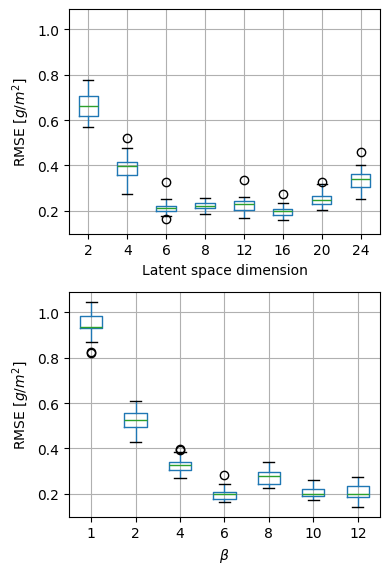
\includegraphics[width=\textwidth]{f04}
  \caption{%
    The neural network was trained to generate samples of two-dimensional ash column mass, \ie the total mass of volcanic ash in a vertical column.
    In this example, a VAE-generated ensemble composed of 12 samples is shown.
    }
  \label{fig:vae_ensemble}
\end{figure*}

\subsubsection{Ensemble mean and spread}
The VAE ability to reproduce sample statistics, such as the ensemble mean and spread (standard deviation), is examined in this section and a few metrics are reported. Figure~\ref{fig:mean} compares the ensemble means of the training ensemble (Fig.~\ref{fig:mean}a) and VAE-generated ensemble comprising 5000 members (Fig.~\ref{fig:mean}b). Ideally, VAE should be able to closely approximate the test dataset (target) to achieve good performances. Deviations from the target are quantified by bias maps. In relative terms, the bias is small for both the training dataset (Fig.~\ref{fig:mean}c) and VAE (Fig.~\ref{fig:mean}d), although the training dataset provides a slightly better estimate of the ensemble mean in general.

\begin{figure*}[htbp]
  \centering
  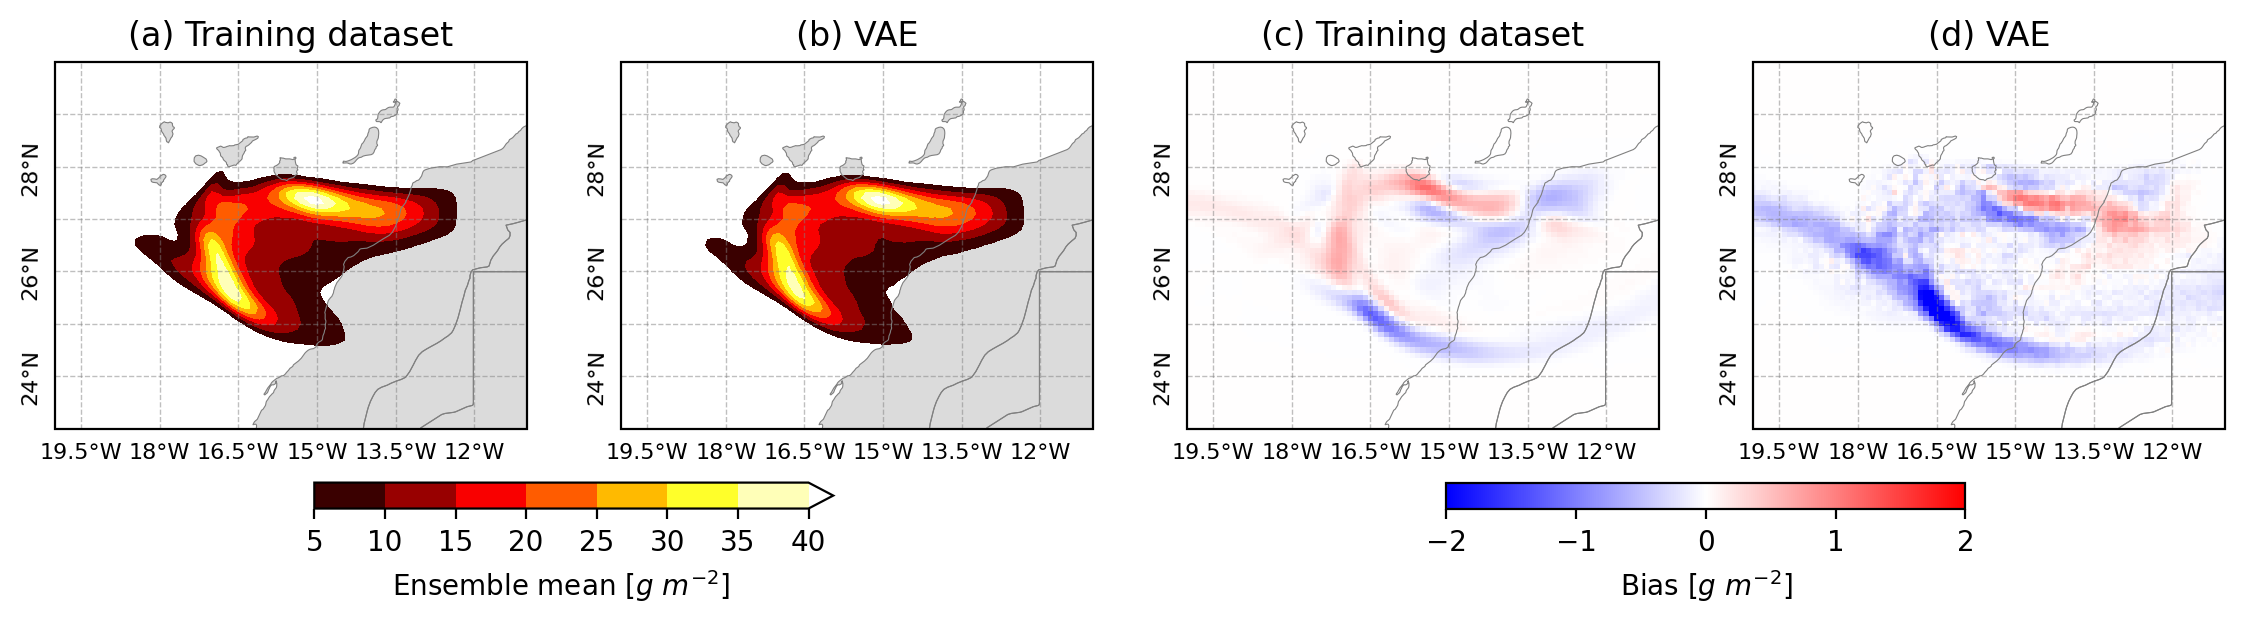
\includegraphics[width=\textwidth]{f05}
  \caption{%
    Ensemble mean maps obtained from the training dataset (a) and a VAE-generated ensemble with 5000 samples (b). 
    The bias maps for the training (c) and VAE (d) ensemble means are computed by subtracting the target (test dataset) corresponding results.
    }
  \label{fig:mean}
\end{figure*}

A summary of the metrics is shown in Table~\ref{tab:metrics}. Metrics are computed for multiple VAE-generated ensembles composed of 5000 samples in order to account for the variability introduced by stochastic sampling. The average over 20 ensembles is reported along with the standard deviation for the uncertainty. The target test dataset is taken as a reference in order to evaluate each of the metrics described in Sect.~\ref{sec:metrics}. The VAE errors measured in terms of the RMSE are twice as high as those evaluated from the training dataset. In relative terms, this represents an error of 1.78\% (training) and $3.4\%$ (VAE) according to the MAPE evaluated from the ensemble mean. In order to avoid divisions by zero and numerical instabilities, the MAPE was actually computed considering only the region where the test dataset is above 5~\unit{g\,m^{-2}} (\ie the range shown in Figs.~\ref{fig:mean}a,b). We can conclude that VAE is properly capturing the first (mean) and second moments (variance) of the distribution, although the training estimations for the ensemble mean and spread are still slightly better.
%
The next section demonstrates that, when larger ensembles are generated, the VAE tends to perform better on statistics more sensitive to sampling errors.

\begin{table}[t]
  \caption{
    A summary of some performance metrics evaluated using the test dataset as the reference target.
    The VAE metrics were averaged over 20 ensembles generated to account for stochastic variability.
    The uncertainty range is given by the standard deviation.
  }
  \label{tab:metrics}
  \begin{tabular}{lccc}
    \tophline
    Metric    & Variable  & Training dataset  & VAE (5000 samples) \\ \middlehline
    RMSE      & Mean      & 0.108             & $0.20  \pm 0.03$   \\
    MBE       & Mean      & 0.001             & $-0.04 \pm 0.02$   \\
    MAPE (\%) & Mean      & 1.784             & $3.4   \pm 0.6$    \\ \middlehline
    RMSE      & Spread    & 0.255             & $0.56  \pm 0.04$   \\
    MBE       & Spread    & -0.004            & $-0.17 \pm 0.01$   \\
    \bottomhline
  \end{tabular}
  \belowtable{ 
    Values are reported in \unit{g~m^{-2}}, except MAPE, which is given as a percentage (\%).
    }
\end{table}

\subsubsection{Probability distributions} \label{sec:res:pd}
An important aspect in hazard and impact assessment is to evaluate exceedance probabilities, \ie the probability that a specific hazardous threshold is exceeded within a given time frame. In the context of ensemble modelling, probability distribution estimations can suffer from sampling errors, particularly when small ensembles are considered. Figure~\ref{fig:exceedance} presents the exceedance probabilities for three different thresholds, demonstrating that the VAE is capable of generating accurate probability distributions as well as realistic samples.
%
In order to examine whether the sampled ensemble provides a good approximation to the target distribution, a few histograms are shown in Fig.~\ref{fig:histograms} at four selected locations, comparing results for the training dataset (left column) and a VAE ensemble with 5000 samples (right column), considering 128 bins between the minimum and maximum values for each location. As expected, the distribution estimated from the training dataset with a small ensemble size ($\ensSize=256$) results in a very noisy distribution, while the VAE distribution provides a good approximation to the test dataset distribution, even for multimodal distributions (\eg, Fig.~\ref{fig:histograms}a).

\begin{figure*}[htbp]
  \centering
  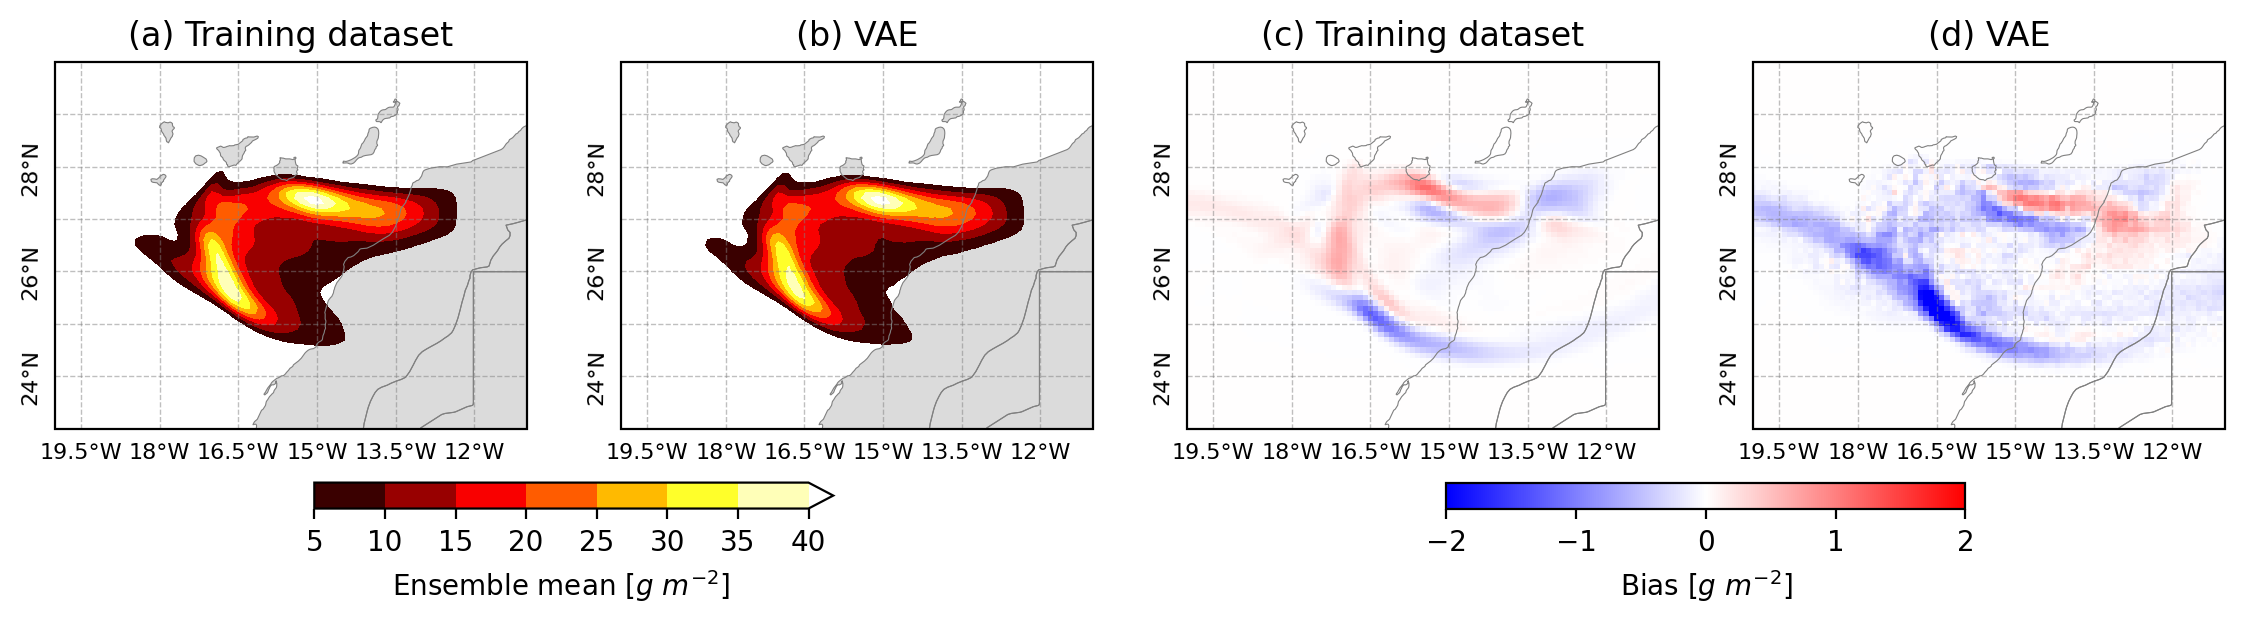
\includegraphics[width=\textwidth]{f06}
  \caption{%
    Exceedance probabilities for three ash column mass thresholds (8, 16 and 20~$g~m^{-2}$ from top to bottom). 
    The probability contours correspond to $2\%$, $25\%$, $50\%$, $75\%$ and $98\%$.
    Results for the training dataset (left column) and a VAE-generated ensemble with 5000 samples (central column) are compared to the test dataset target (right column).
    }
  \label{fig:exceedance}
\end{figure*}

\begin{figure*}[ht]
  \centering
  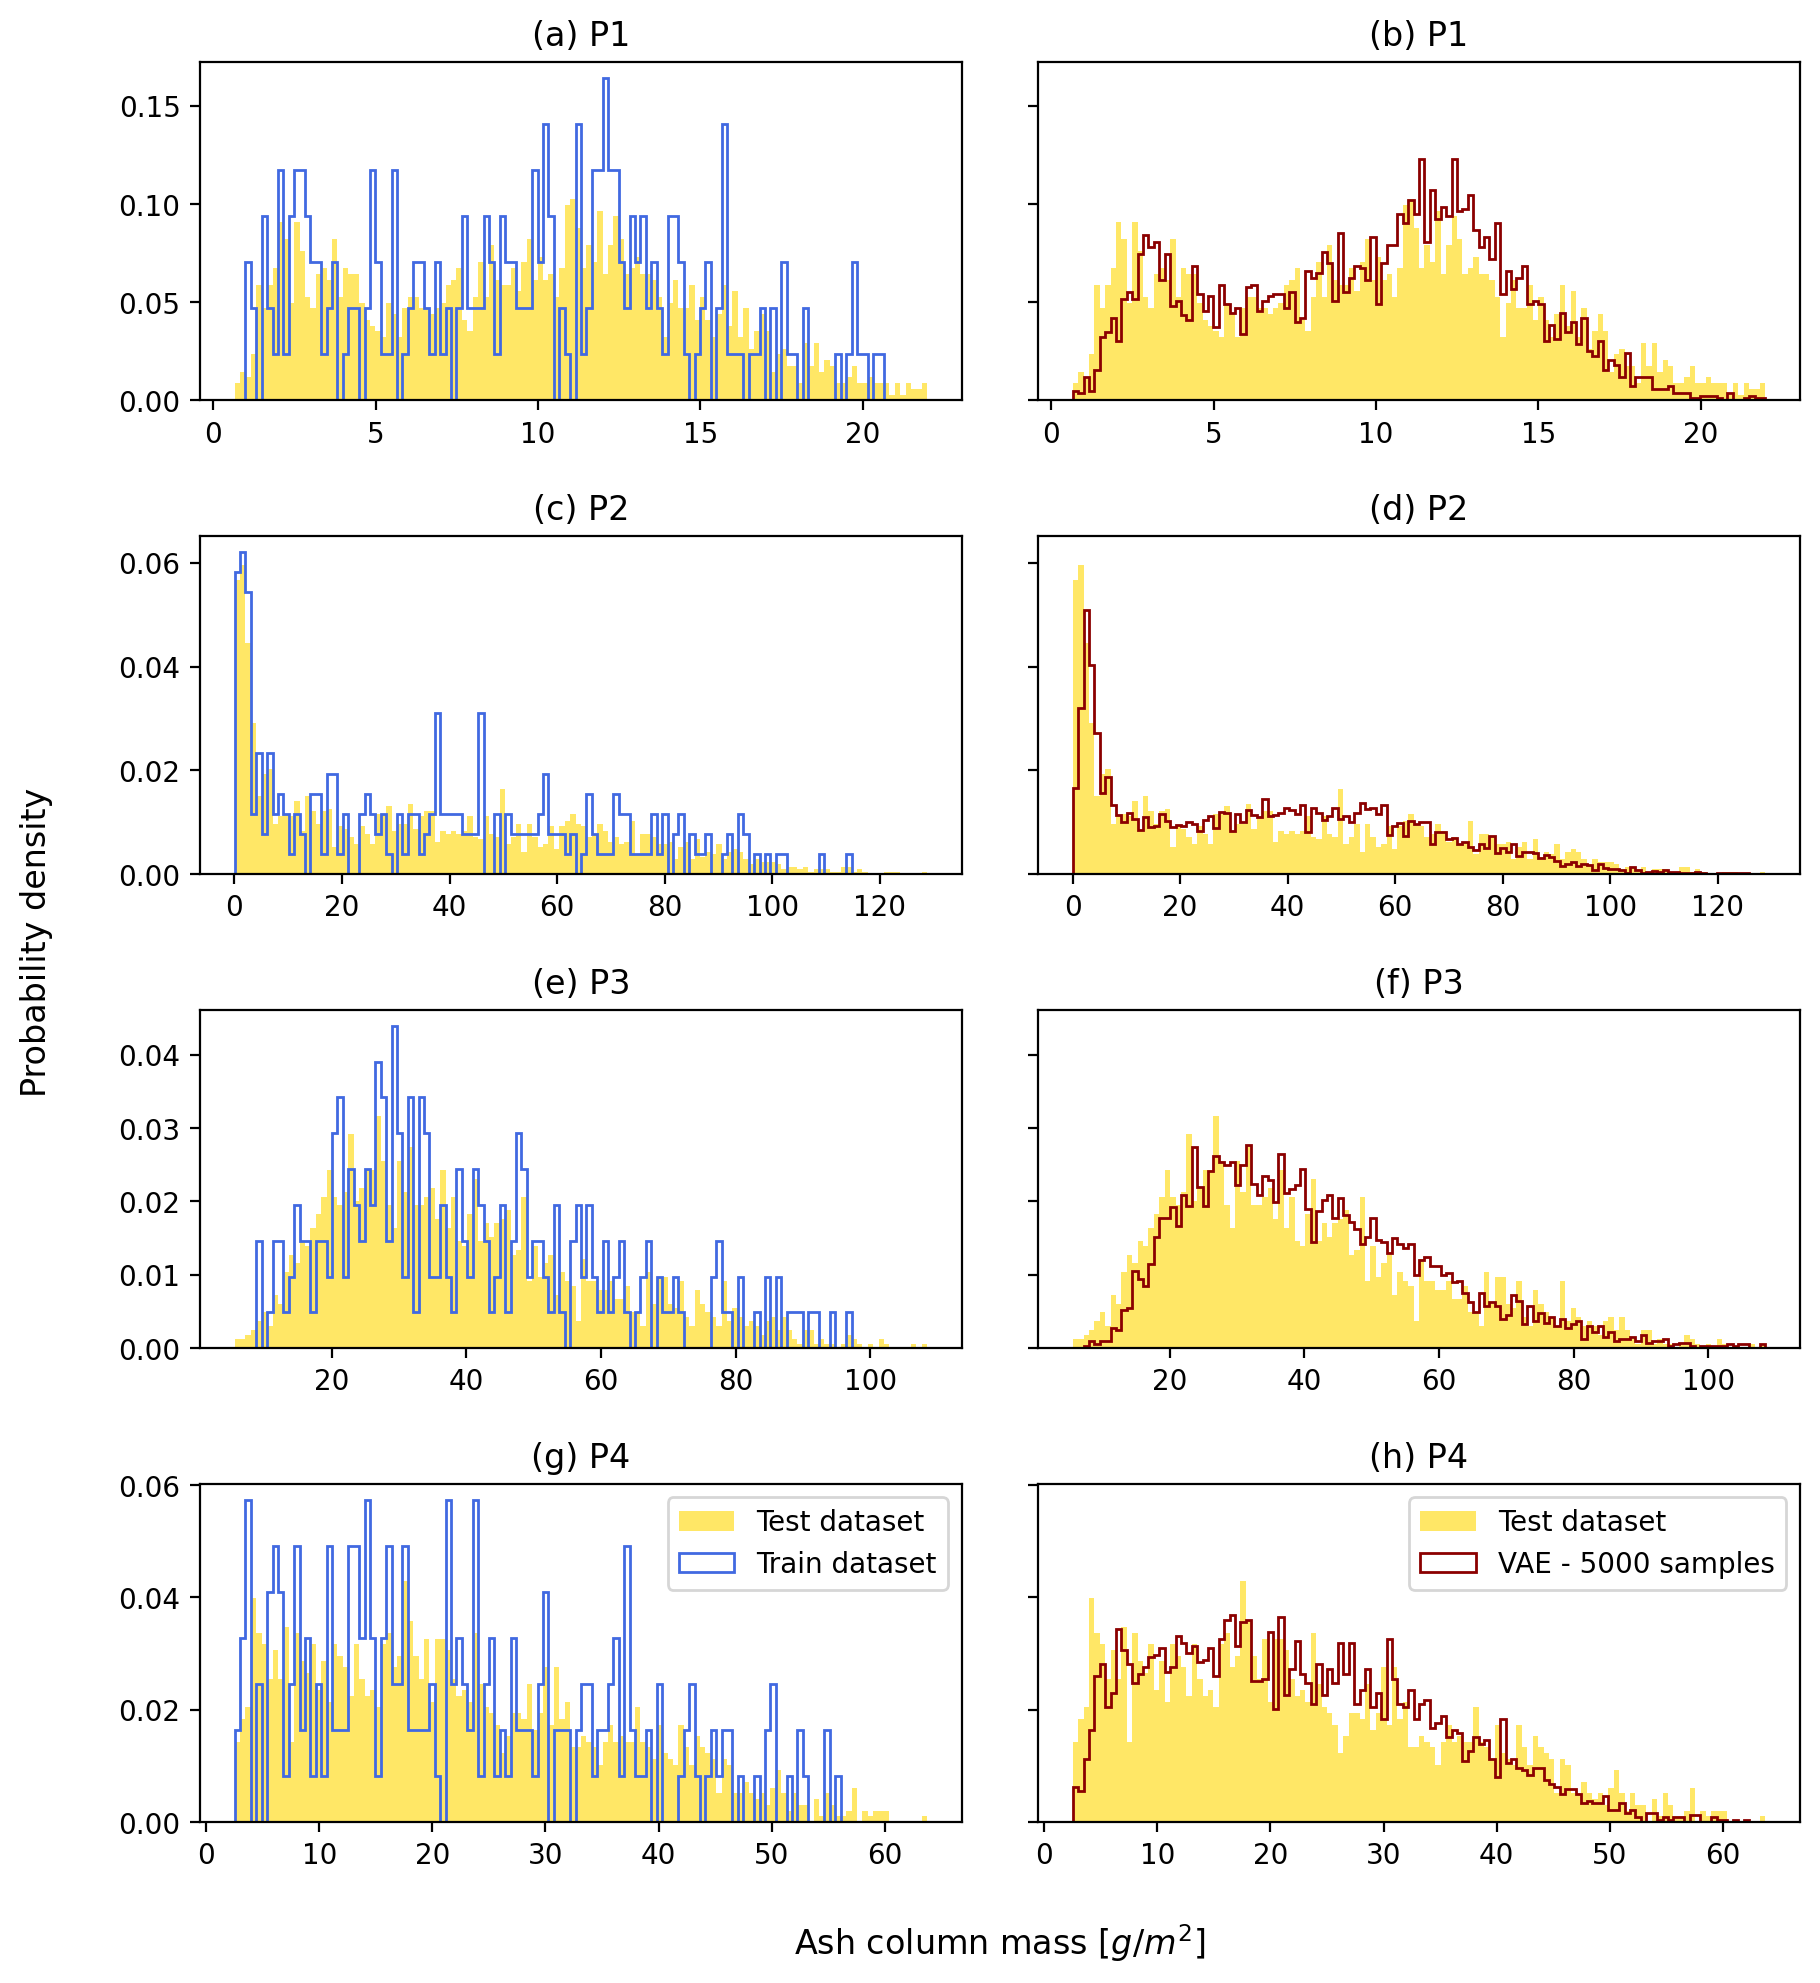
\includegraphics[width=0.8\textwidth]{f07}
    \caption{
      Histograms for the training dataset (256 samples, left column) and a 
      VAE-generated ensemble (5000 samples, right column) at different locations. 
      The results are compared against the test dataset (2048 samples), 
      assumed to be the reference target (yellow shaded area). 
      For illustrative purposes, four sampling locations were selected: 
      P1 at 15.5\degree\,W, 26.3\degree\,N \textbf{(a, b)}; 
      P2 at 16.8\degree\,W, 25.9\degree\,N \textbf{(c, d)}; 
      P3 at 15.0\degree\,W, 27.3\degree\,N \textbf{(e, f)}; and 
      P4 at 15.5\degree\,W, 27.4\degree\,N \textbf{(g, h)}.
    }
  \label{fig:histograms}
\end{figure*}

Naturally, the VAE capacity to approximate the distribution depends on the number of samples generated. In order to assess the quality of the approximation for different amounts of samples, the JS divergence was computed from discrete probability distributions using~\eqref{eq:js}. Specifically, $JSD$ was obtained from histograms with a fixed range (128 bins between 0 and 40 $g~m^{-2}$) for each grid cell. As a measure of the worst-case conditions, the 99th percentile of the grid‐cell values is reported in Fig.~\ref{fig:js_divergence}, taken as a robust estimation of the maximum $JSD$ over the domain. The results for multiple VAE-generated ensemble sizes are compared with the training dataset. As expected, VAE improves the training distribution only for large ensemble sizes ($\ensSize\gtrsim 256$), reaching an asymptotic value of approximately $JSD \sim 0.042$, which represents a 2.6x improvement over the corresponding training metric ($JSD=0.11$).

\begin{figure}[htbp]
  \centering
  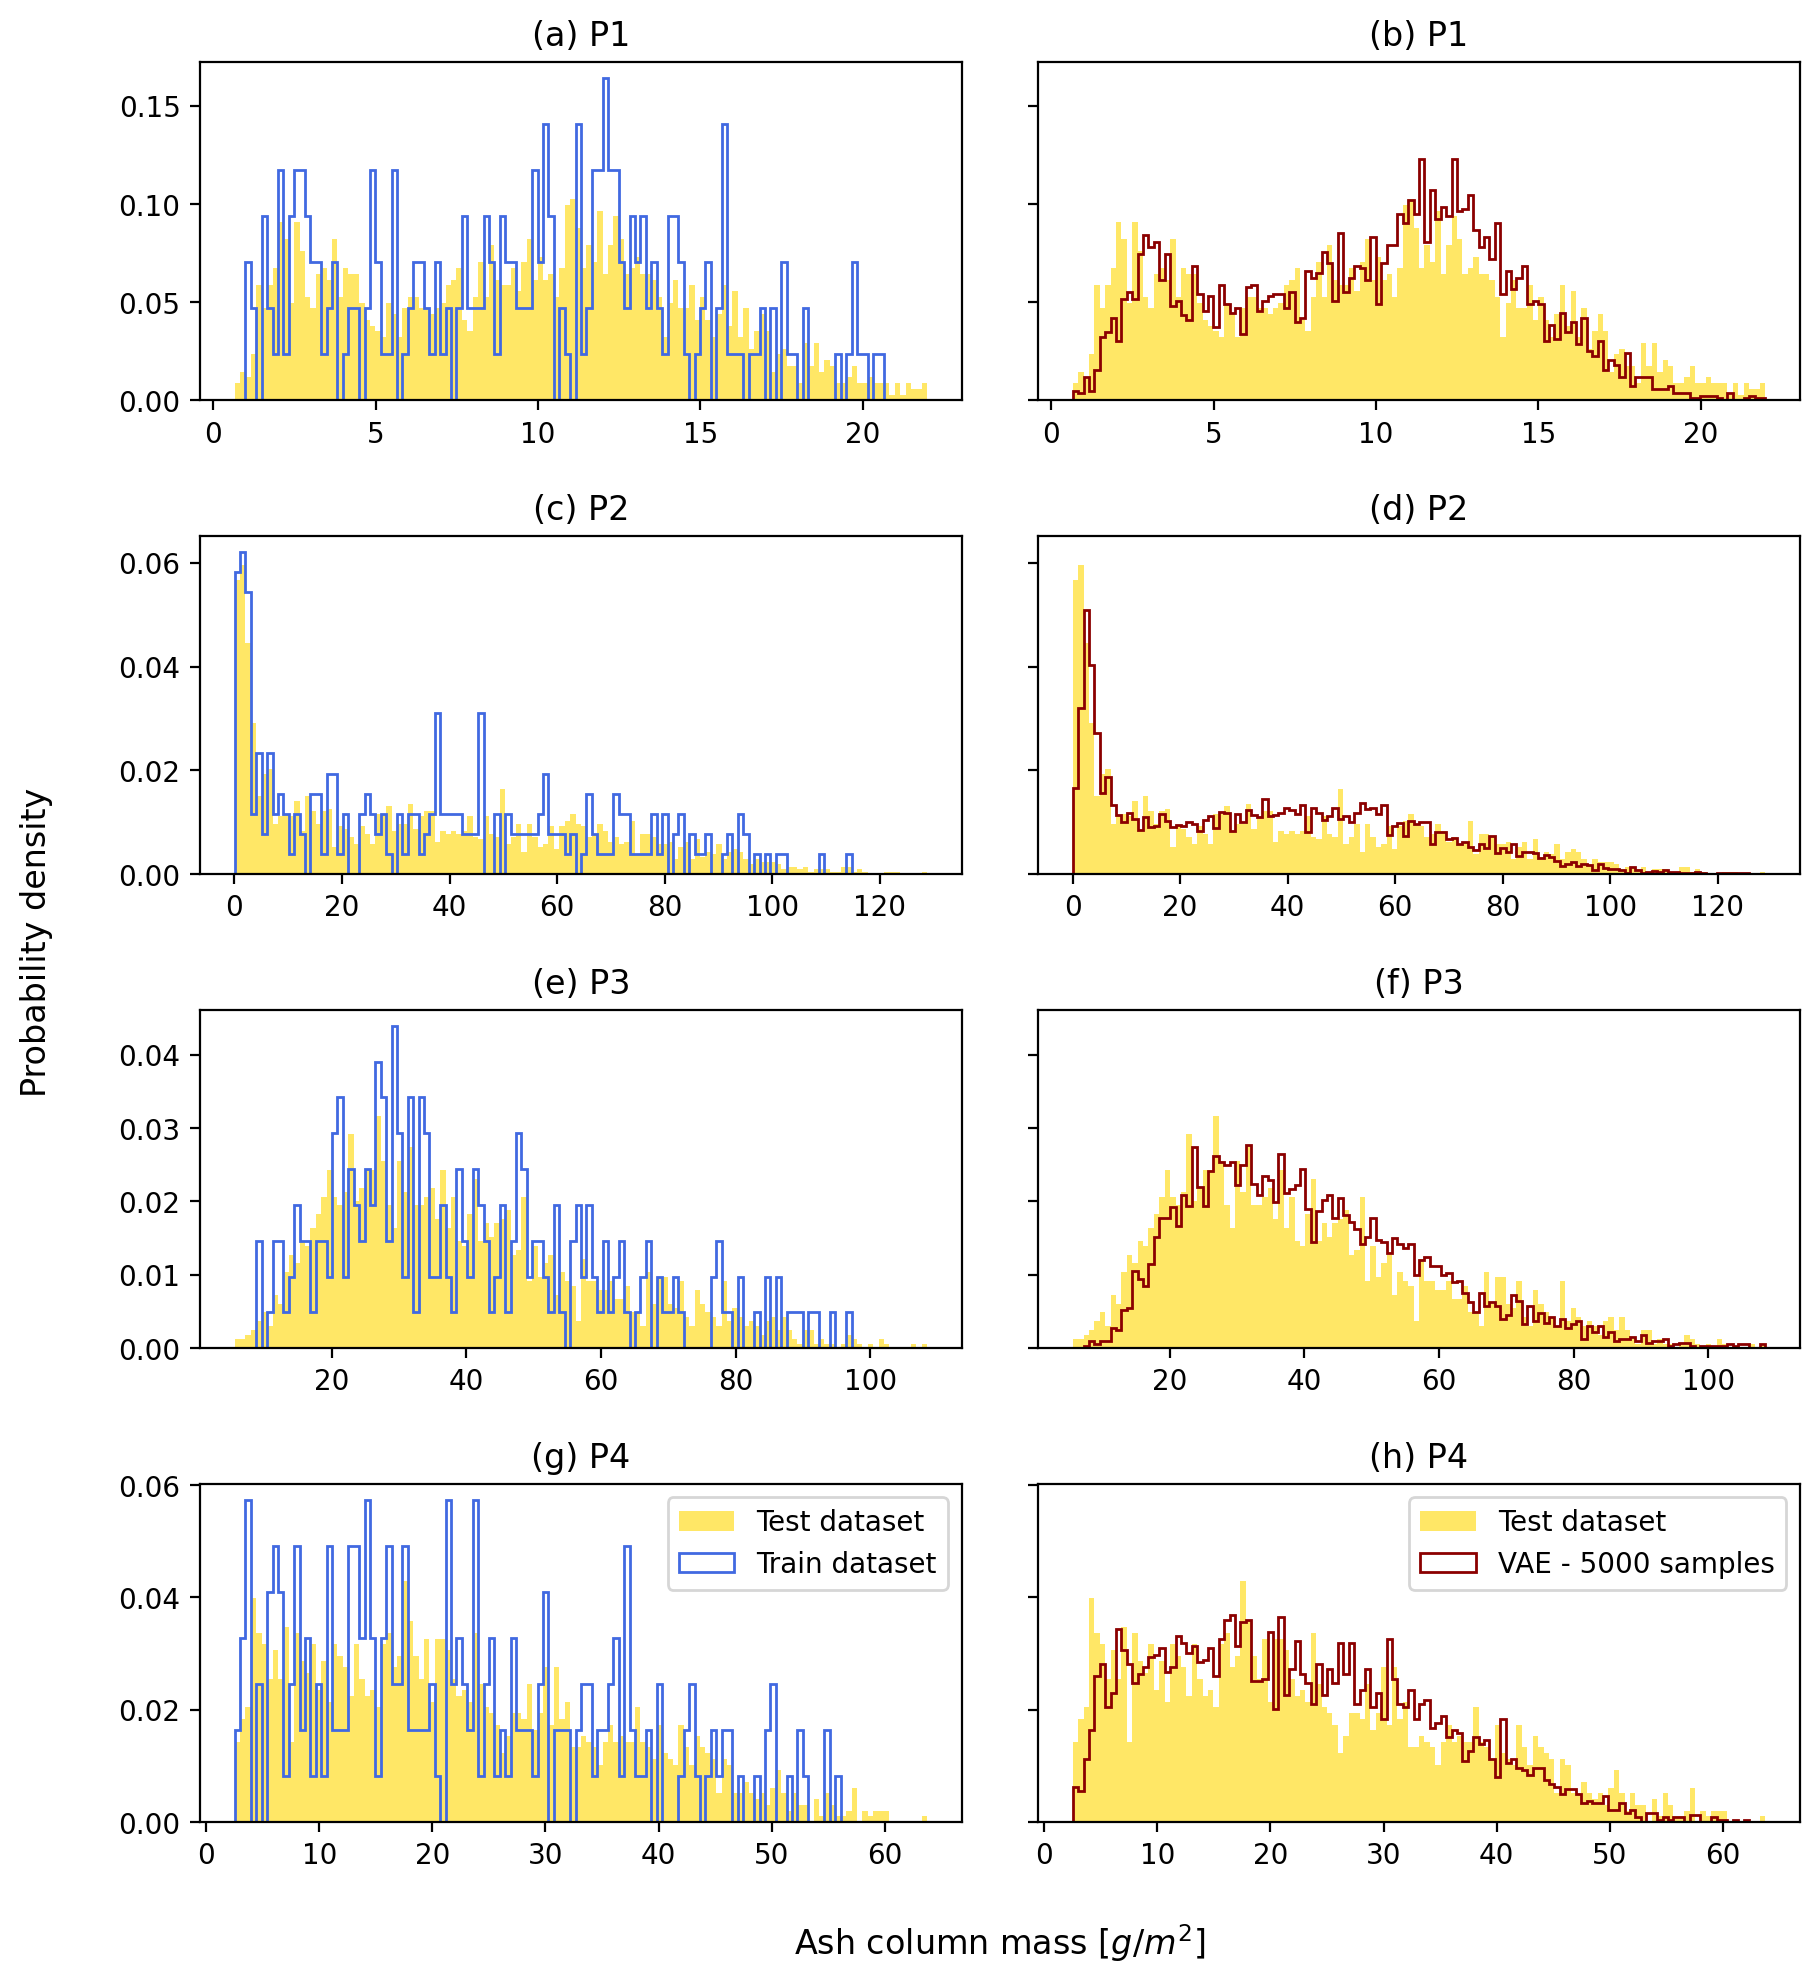
\includegraphics[width=0.45\textwidth]{f08}
  \caption{%
    The Jensen-Shannon (JS) divergence was computed for each grid cell 
    considering different sizes of the VAE-generated ensemble.
    The 99th percentile is reported as a worst-case measure of performance.
    Low values indicate a good approximation to the actual probability distribution. 
    The result for the training dataset is also indicated for reference.
    }
  \label{fig:js_divergence}
\end{figure}

\subsubsection{Isotropic power spectrum} \label{sec:psd}
%
% PSD, general description
%
The isotropic power spectrum, \ie the radially averaged two-dimensional Power Spectral Density (PSD), was computed using \eqref{eq:psd}. Figure~\ref{fig:psd} presents the results for the test dataset and VAE, averaged over multiple ensemble realizations (each ensemble with $\ensSize=5000$ samples). It is worth noting that, instead of the classical energy cascade spectrum proportional to $k^{-5/3}$, the test dataset exhibits an exponential decay (solid red line), likely due to the diffusion processes introduced by the dispersal model FALL3D. The generative model, with a strongly regularized latent space, reproduces well the large scales but fails at smaller scales, as shown in Fig.~\ref{fig:psd} (green triangles).
%
% High frequency noise
%
The isotropic power spectrum deviates from the exponential decay for wavenumbers above $\sim 0.3~\Delta x^{-1}$, approximately, where $\Delta x$ is the grid size. In other words, the VAE is unable to reproduce variability at spatial scales below $\sim 3~\Delta x$. The flat high-wavenumber tail in the 2D power spectrum seems to be related to the convolutional kernel size used in this work (\ie, $3\times 3$) and the limitations of the decoder upsampling. Our decoder architecture is based on transposed convolution layers, and it is widely known that transposed convolutions usually lead to chequerboard artifacts. Actually, this effect can also be observed from the bias map of the ensemble mean (Fig.~\ref{fig:mean}d), where a noisy pattern with relatively low intensity and high-frequency structure can be identified.
%
% Kernel size
%
A new neural network was trained using a larger kernel size ($5\times 5$) in order to investigate whether it yields to a more effective low-pass filtering (blue crosses in Fig.~\ref{fig:psd}). Although the background noise was reduced slightly, the results remained almost identical. Future work should investigate more advanced neural network architectures to better address this limitation.
%
% High beta
%
Finally, this behaviour is consistent with the disentangled latent representation enforced by a high value of the $\beta$ hyperparameter (see Fig.~\ref{fig:boxplot}). In fact, the VAE learns a smooth, structured encoding that preserves the dominant generative factors while filtering out small-scale variations that would otherwise help reduce the reconstruction error. The effects of this strongly regularized latent space are also visible in the spectral analysis. While the VAE successfully reproduces the low-frequency components associated with large-scale structures, it systematically underestimates the high-frequency content responsible for fine-scale details. 

\begin{figure}[htbp]
  \centering
  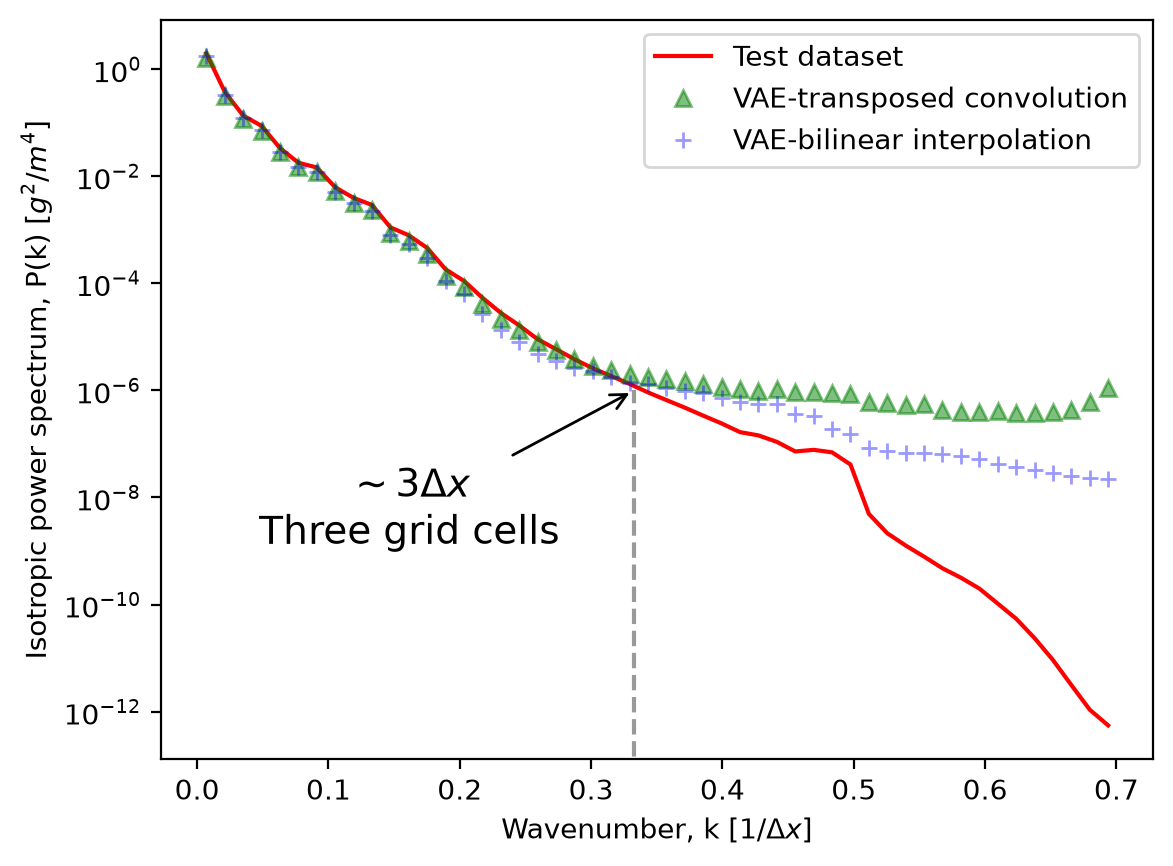
\includegraphics[width=0.45\textwidth]{f09}
  \caption{%
    The isotropic power spectrum, \ie radially averaged 
    two-dimensional Power Spectral Density (PSD), 
    reveals inconsistencies in the spatial structure of 
    the VAE-generated samples. 
    The generative model reproduces large scales but fails 
    at scales smaller since the VAE is introducing 
    artificial noise for large k. Since the wavenumber 
    is expressed in terms of the grid size, $\Delta x$, 
    we can conclude that the VAE is unable to reproduce 
    the variability over spatial scales below 
    $\sim 3~\Delta x$, approximately. 
    }
  \label{fig:psd}
\end{figure}

\subsection{Latent-space assimilation of satellite observations} \label{sec:res:da}
This section shows the results of the latent-space data assimilation for the Etna experiment (see Sect.~\ref{sec:etna-experiment}). Figure~\ref{fig:etna2018}a shows the ensemble mean of the model prior ($\ensSize=128$), \ie the ensemble of two-dimensional ash column mass at 18:00~UTC simulated with the dispersal model FALL3D. The corresponding satellite retrievals from SEVIRI are shown in Fig.~\ref{fig:etna2018}b. The relatively complex spatial structure of the observed plume results from a pronounced clockwise rotation (veering) of its trajectory during the initial phase of the eruption. This change in flow direction is not captured by the driving meteorological dataset, which leads FALL3D to simulate ash transport under a largely uniform directional flow. Consequently, this case represents a challenging test for the data assimilation methodologies.

\begin{figure}[htbp]
  \centering
  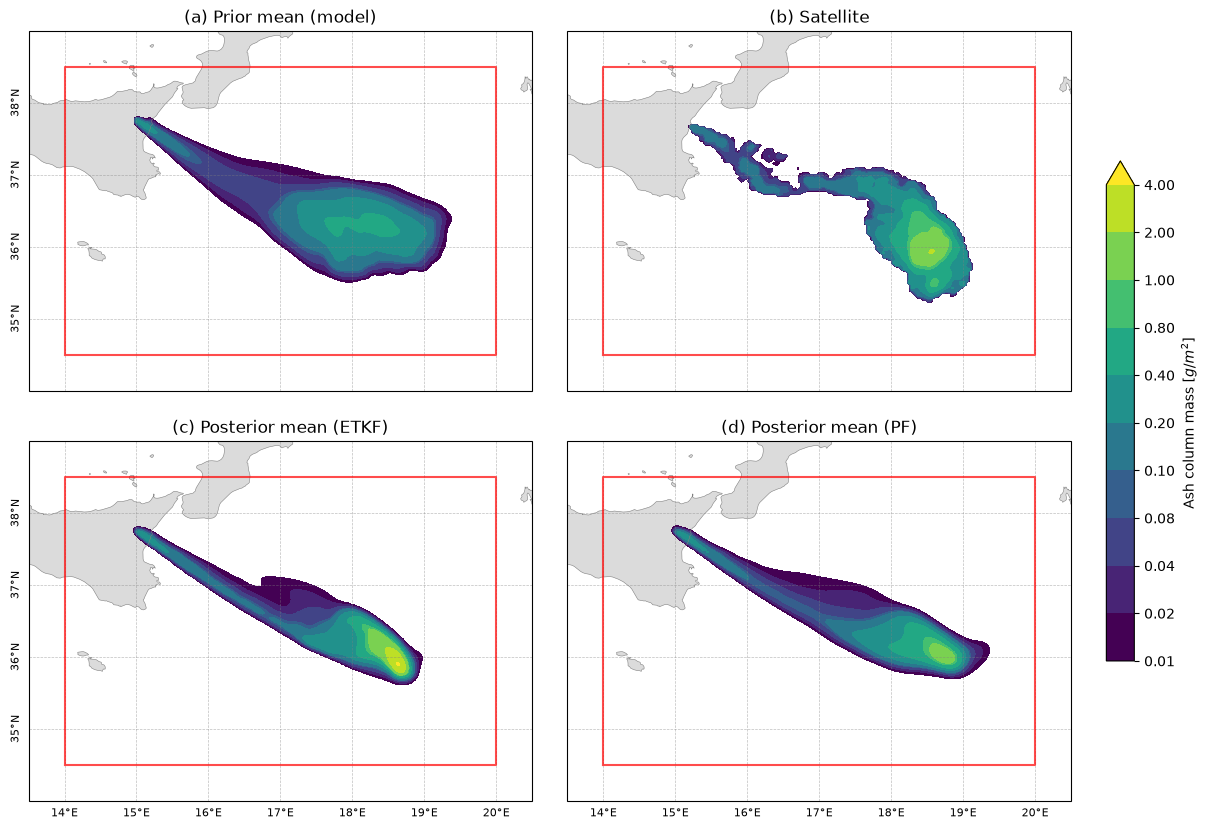
\includegraphics[width=0.9\textwidth]{f10}
  \caption{%
    Spatial distribution of ash column mass at 18:00~UTC for the Etna 24 December 2018 case for 
    \textbf{(a)} the ensemble mean of the model prior, 
    \textbf{(b)} the SEVIRI satellite retrievals, 
    \textbf{(c)} the ETKF posterior ensemble mean, and 
    \textbf{(d)} the PF posterior ensemble mean. 
    The red box shows the FALL3D model domain extent.
    }
  \label{fig:etna2018}
\end{figure}

\subsubsection{VAE prior}
The simulated model prior is used to train a new VAE, which is subsequently used to generate an augmented ensemble (VAE prior) by sampling from the latent space. The same procedure and neural network architecture used for the synthetic experiments are employed for the Etna experiment, with a few exceptions:
(i) to accommodate the increased size of the input data, the latent dimension was increased to $\latentDim=32$ and a new convolutional layer was added to both the encoder and decoder;
(ii) we found that the checkerboard pattern can be reduced by replacing transposed convolutional upsampling with bilinear interpolation; and 
(iii) rather than sampling the latent variables from a standard normal distribution, the latent vectors are sampled from a multivariate normal distribution,
\begin{equation}
\mathbf{z}_i \sim \mathcal{N}(\boldsymbol{\mu}, \boldsymbol{\Sigma}),
\end{equation}
where $\boldsymbol{\mu}$ and $\boldsymbol{\Sigma}$ are estimated from the latent representations of the training ensemble. The VAE prior is then generated by sampling $\ensSize=4096$ latent vectors $\mathbf{z}_i$ from this distribution and then decoded to obtain the VAE prior in the original ash column mass space.

The agreement with the satellite observations is evaluated using the metrics defined in Sect.~\ref{sec:metrics}. Table~\ref{tab:rmse_metrics} compares the model prior and VAE prior against the satellite observations. The metrics are computed for every ensemble member and the ensemble average is reported. Both model and VAE ensembles show very similar performance across all metrics, with the VAE prior yielding slightly better RMSE, RMSLE and Pearson correlation. These results indicate that the VAE-generated ensemble preserves the main characteristics of the model prior relevant to the comparison with observations. The results are also consistent with the previous analysis, showing that the VAE can generate samples that are statistically comparable to those produced by the physics-based FALL3D model.
%
% Concluding remarks
%
These results provide a baseline for assessing the impact of data assimilation in the next section, while also demonstrating that the VAE-generated ensemble provides a suitable prior for subsequent data assimilation experiments.

\begin{table}[htbp]
    \centering
    \caption{Metrics used to quantify agreement with observations for the Etna data assimilation experiment.}
    \label{tab:rmse_metrics}
    \begin{tabular}{lcccc}
        \tophline
         & Prior   & Prior & Posterior & Posterior \\
         & (model) & (VAE) & (ETKF)    & (PF) \\ \middlehline
        RMSE & 180.317 & 173.562 & 145.696 & 126.903 \\
        RMSLE & 1.561 & 1.491 & 1.228 & 1.210 \\
        Pearson correlation & 0.315 & 0.339 & 0.700 & 0.667 \\
        POD & 0.278 & 0.274 & 0.381 & 0.378 \\
        Jaccard index & 0.229 & 0.227 & 0.325 & 0.333 \\
        \bottomhline
    \end{tabular}
\end{table}

\subsubsection{Data assimilation experiments}
%
% Spatial results
%
The analysis ensemble means obtained with the ETKF (Fig.~\ref{fig:etna2018}c) and PF (Fig.~\ref{fig:etna2018}d) show that both the intensity and location of the maximum are corrected relative to the prior. However, the analysis ensembles retain the lack of representation of the veering and wind shear present in the prior, resulting in an almost unidirectional and less extended plume. This illustrates an important limitation of the assimilation: the analysis can preferentially select and combine ensemble members that are more consistent with the observations, but cannot recover spatial structures that are not represented in the prior ensemble.
%
% Quantitative improvement
%
The impact of the assimilation can be assessed in terms of the evaluation metrics reported in Table~\ref{tab:rmse_metrics}. These diagnostics are not intended as an independent validation, but rather to characterize the adjustment of the prior ensemble towards the observational constraints. The agreement with the observations improves for all metrics following assimilation. The RMSE is reduced by 16\% (ETKF) and 27\% (PF) relative to the VAE prior, while the RMSLE decreases by 18\% (ETKF) and 19\% (PF). The Pearson correlation approximately doubles for both methods. A larger relative improvement is obtained for the categorical metrics: the ETKF increases the POD and Jaccard index by 39\% and 43\%, respectively, while the corresponding increases for the PF are 38\% and 47\%. Overall, both assimilation approaches consistently adjust the ensemble towards the observations, with comparable performance across the different metrics considered.

%
% Ensemble spread
%
The impact of the assimilation can also be assessed in terms of the ensemble spread. The ensemble spread quantifies the dispersion of the ensemble members around the mean and is computed as the ensemble standard deviation at each element, averaged over all elements. The resulting spreads for the prior and posterior ensembles are reported in Table~\ref{tab:spread_metrics}. This metric is evaluated both in physical space and in latent space.
%
% PF collapse
%
The spread reduction in latent space is 10\% (ETKF) and 42\% (PF). The substantially lower PF spread results from particle-filter degeneracy, with nearly all posterior probability concentrated on only two particles. Kernel perturbation is subsequently used to increase ensemble diversity, with a regularization factor of $h=0.2$ (see Sect.~\ref{sec:pf}). Interestingly, the spread reduction in physical space is more pronounced for the ETKF (77\%) than for the PF (70\%), despite the substantially larger reduction observed for the PF in latent space.

\begin{table}[htbp]
    \centering
    \caption{Ensemble spread of the prior and posterior ensembles in latent and physical space}
    \label{tab:spread_metrics}
    \begin{tabular}{lrr}
        \tophline
        ~              & Latent-space spread & Physical-space spread \\ \middlehline
        VAE Prior      & 0.999 & 33.974 \\
        ETKF Posterior & 0.899 & 7.804 \\
        PF Posterior   & 0.582 & 10.351 \\
        \bottomhline
    \end{tabular}
\end{table}

%
% Latent-space distributions
%
The latent-space distributions of the prior and posterior ensembles are shown in Fig.~\ref{fig:latent-distribution} for selected pairs of latent dimensions, together with their corresponding histograms. In general, the prior distribution is well approximated by the standard normal distribution, as expected from the VAE construction. The ETKF produces a Gaussian-like posterior, whereas the PF analysis is clearly bimodal, reflecting the concentration of the posterior weights on two particles during the initial filter update. The subsequent kernel perturbation broadens these two modes, restoring some variability.

\begin{figure}
    \centering
    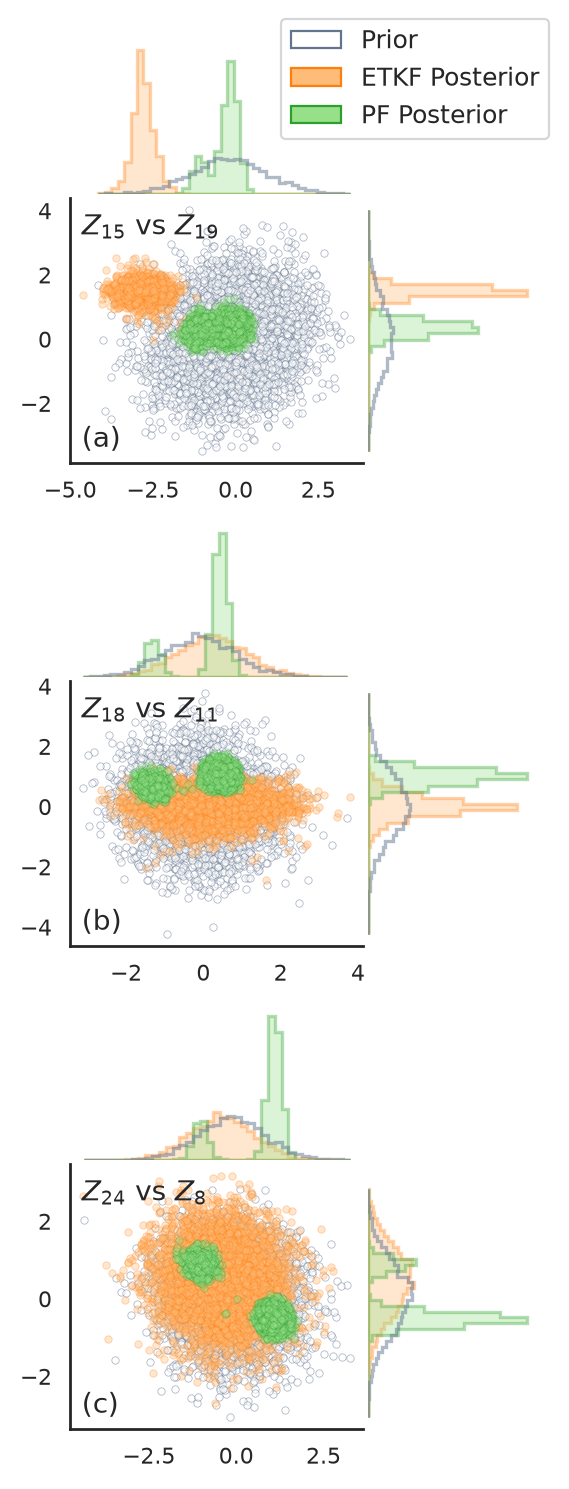
\includegraphics[width=0.42\linewidth]{f11.png}
    \caption{
        Latent-space distributions of the prior and posterior ensembles from the data assimilation experiments. Three selected pairs of latent dimensions are shown for illustration. The ensembles, each comprising 4096 members, are: VAE prior (white), ETKF posterior (orange), and PF posterior (green).
        }
    \label{fig:latent-distribution}
\end{figure}


\subsection{Discussion} \label{sec:discussion}
%
% General remarks
%
In this work, the VAE is viewed as a complement to the physics-based model. Making use of an ensemble of a few hundred simulations, the VAE learns a compact, low-dimensional representation of the complex, high-dimensional variability captured by the physics-based simulations. This representation provides an alternative space in which the structure of the ensemble can be analysed and manipulated. 

%
% Ensemble augmentation
%
Sampling in the latent space to generate an augmented ensemble is the most straightforward application of this methodology. Although it does not introduce new physical knowledge, the VAE can generate a much larger number of realizations at very low computational cost during inference, while retaining variability that is statistically consistent with that captured by the physics-based simulations.
%
% Computational cost
%
It is interesting to consider whether this methodology can be computationally efficient, accounting for both training and inference, when generating ensembles larger than the training ensemble. However, the answer depends on the available computational resources, the cost of the physics-based model, the total simulation time, and the ensemble size, among other factors. As an illustrative example, let's consider the Etna experiment, which is the most computationally demanding case presented here. The 128 FALL3D simulations were run on the accelerated partition of MareNostrum5 using 128 NVIDIA Hopper GPUs, requiring approximately 1 GPU-hour in total. In contrast, VAE training was performed on a laptop using a single RTX 5000 Ada Generation NVIDIA GPU and required only $5.83 \times 10^{-3}$ GPU-hours. In this experiment, the forecast period was limited to 8~h; extending the forecast period would further increase the relative cost of the numerical simulations. Most importantly, the approach substantially reduces the computational resources required to generate large ensembles; for example, the simulations for the synthetic experiment on the LUMI supercomputer required at least 2,048 GPUs. Of course, these examples do not allow us to draw general conclusions about the relative efficiency of augmenting an ensemble with a VAE versus explicitly simulating larger ensembles, as the computational cost depends on the type of model and the available computational resources. However, computational efficiency is arguably not the main advantage of the proposed approach.

%
% Sampling errors
%
This methodology presented in this work also offers potential advantages beyond ensemble augmentation. Increasing the ensemble size can reduce sampling errors and improve the estimation of statistical quantities that are particularly sensitive to small ensemble sizes, such as exceedance probabilities and other measures of uncertainty. Such estimates are particularly relevant for probabilistic hazard assessment and decision-making in crisis management. For example, as shown in Sect.~\ref{sec:res:pd}, the VAE provides a better approximation to the reference distribution than the training ensemble in terms of the Jensen--Shannon (JS) divergence when the ensemble size exceeds the number of numerical simulations used for training.

%
% Sample generation
%
Additionally, due to the generative nature of the VAE, instead of simply duplicating or resampling existing numerical simulations, as in a bootstrap approach, new realizations absent from the original dataset can be generated. This could potentially lead to a richer statistical representation of the variability captured by the physics-based model, particularly if some of the generated realizations correspond to regions of the distribution that are poorly represented in the training ensemble. This interpretation is consistent with the results presented in Sect.~\ref{sec:da}, where the VAE-generated ensemble shows better agreement with the observations than the model prior in terms of RMSE, RMSLE, and Pearson correlation (Table~\ref{tab:rmse_metrics}).

%
% Operations in the latent space
%
Most importantly, the learned representation enables different operations to be performed in a substantially lower-dimensional space, including data assimilation, clustering, perturbation, conditional sampling, and other statistical techniques. These capabilities provide an excellent opportunity for further research. In this study, we explore two latent-space data assimilation approaches that, in the formulation adopted here, would not be directly applicable in the original physical space.
%
% Data assimilation
%
The assimilation experiments demonstrate the feasibility of performing data assimilation directly in the VAE latent space. Both the ETKF and PF adjust the augmented prior towards the satellite observations, improving the agreement across all considered evaluation metrics and reducing the ensemble spread without an excessive loss of ensemble variability. Although the two assimilation approaches produce markedly different posterior distributions in latent space, their resulting posterior ensembles in physical space are relatively similar.
%
% Particle filter collapse
%
The particle-collapse problem of the PF was not fully resolved, as the posterior distribution remained concentrated around two particles, resulting in a bimodal distribution after the perturbation introduced by the kernel regularization. Applying such a naive perturbation directly in the physical space for a nonlinear model would result in states that are inconsistent with the model dynamics. Instead, perturbing in latent space takes advantage of the learned mapping, allowing perturbed particles to be mapped back to physical space while retaining consistency with the physics-based simulations. This clearly illustrates one of the advantages of performing operations directly in the latent space.

Overall, the results presented in Sect.~\ref{sec:res:da} demonstrate that latent-space data assimilation can effectively incorporate satellite observations to correct a large VAE-generated ensemble of two-dimensional volcanic ash column mass. Future research is needed to assess whether the methodology can be extended to the full three-dimensional concentration field and multiple particle classes, which will require adapting the neural network architecture to the increased dimensionality of the problem. This extension would be an important step for enabling multiple assimilation cycles and, ultimately, supporting operational forecasting.
\conclusions \label{sec:conclusions}
%
% Short summary
%
This study explored the potential of a hybrid strategy for volcanic-cloud modelling based on the integration of generative AI with physics-based simulations. A Variational Autoencoder (VAE) was trained on a relatively small ensemble of numerical simulations to learn a compact, low-dimensional representation of the high-dimensional problem. This methodology offers several potential advantages, including the generation of large ensembles at very low computational cost, the reduction of sampling errors and improved estimation of ensemble statistics, the generation of new samples beyond those contained in the training dataset, and the ability to perform statistical operations in a substantially lower-dimensional space, including latent-space data assimilation.

%
% Main results
%
Two numerical experiments have been presented. A first synthetic experiment assessed the consistency of the VAE-generated ensemble using a controlled case characterized by multiple qualitatively different solutions, testing the ability of the VAE to capture this variability. Even when no new physical knowledge is introduced by a VAE-augmented ensemble, it provides a good statistical approximation of the reference distribution and generates fields that are statistically consistent with the underlying physical model, particularly at large spatial scales. The results also highlight limitations in the representation of smaller-scale spatial structures.
%
However, the reconstruction error is smaller than the errors introduced by the numerical model itself. In the second  experiment, the 24 December 2018 Etna eruption was modelled and the VAE-augmented ensemble was compared with satellite retrievals. The agreement with observations was found very similar for the numerical and VAE-augmented ensembles, with the latter yielding better RMSE, RMSLE, and Pearson correlation coefficients, suggesting that the generation of new samples can lead to a better statistical representation of forecast uncertainty.
%
The Etna experiment was also used to provide a proof-of-concept demonstration of latent-space data assimilation methodologies. A two-dimensional estimation problem was solved by assimilating satellite retrievals in the VAE latent space. The analysis ensemble showed improved agreement with the observations across all evaluated metrics, while significantly reducing the ensemble spread and retaining the ability to represent the spatial variability of the volcanic cloud and the physical consistency with the simulated prior. 

%
% Final summary
%
In summary, this work represents a first proof of concept based on a relatively simple neural architecture and an elementary data assimilation methodology. The results demonstrate the potential of the formulation, while highlighting the need for further research to assess its robustness and applicability across different eruption scenarios. Future work should extend the methodology to three-dimensional fields, explore more advanced generative models and assimilation approaches, and evaluate their performance against state-of-the-art DA methods and independent observations, ultimately assessing their potential implications for operational forecasting.

\codeavailability{
  FALL3D v9.1 is available under the version 3
  of the GNU General Public License (GPL) at
  \url{https://gitlab.com/fall3d-suite/fall3d/} and 
  \url{https://doi.org/10.5281/zenodo.17737081}
  \citep{folch2020,prata2021}.
  %
}

\authorcontribution{
  Conceptualisation, L.M., M.T.; %
  Methodology, L.M.; %
  Software, L.M., A.F., H.P.; %
  Resources, L.M.; %
  Writing---original draft, L.M.; %
  Writing---review and editing, L.M., A.F., H.P., M.T.; %
  Visualisation, L.M.; %
  Supervision, A.F.; %
  Funding Acquisition, A.F.
  %
  All authors have read and approved the final version of the manuscript.
}

\competinginterests{The authors declare that they have no conflict of interest.} 

\begin{acknowledgements}
  Funded by the European Union. This work has received funding from the European High Performance Computing Joint Undertaking (JU) and Spain, Italy, Iceland, Germany, Norway, France, Finland and Croatia under grant agreement No 101093038, ChEESE-2P, project PCI2022-134973-2 funded by MCIN/AEI/10.13039/501100011033 and by the European Union NextGenerationEU/PRTR.
  %
  Computational resources were provided by the LUMI supercomputer through the EuroHPC Joint Undertaking (project EHPC-DEV-2025D10-040) and MareNostrum 5 ACC supercomputer through the EuroHPC Joint Undertaking (project EHPC-REG-2024R02-128). LUMI is hosted by CSC - IT Center for Science and  MareNostrum-5 is hosted by the Barcelona Supercomputing Center (BSC).
  %
  We gratefully acknowledge Stefano Corradi for supplying the satellite retrieval data of the Etna eruption used in this work.
  %
  Finally, we also thank the two anonymous reviewers for their valuable feedback and suggestions.
\end{acknowledgements}

%% REFERENCES
\bibliographystyle{copernicus}
\bibliography{references.bib}

\end{document}
